\documentclass[aspectratio=169,t]{beamer}
\usefonttheme[onlymath]{serif}
\usepackage[utf8]{inputenc}
\usepackage{graphicx}
\usepackage{subcaption}
\usepackage{color}
\usepackage{graphicx}
\usepackage{fancybox}
\usepackage[vlined]{algorithm2e}
\usepackage{anyfontsize}
\usepackage{standalone}
\usepackage{tikz}
\usetikzlibrary{shapes,arrows.meta}
\tikzset{%
	>={Latex[width=2mm,length=2mm]},
	%Colors
	blackStyle/.style = {draw=black, fill=lightgray},
	tealStyle/.style = {draw=MyTeal, fill=MyLtTeal},
	coralStyle/.style = {draw=MyCoral, fill=MyLtCoral},
	sandStyle/.style = {draw=MySand, fill=MyLtSand},
	%Base Styles
	base/.style = {
		draw=black, fill=white, thick,
		text centered, font=\sffamily, inner sep=.2cm},
	baseVar/.style = {base, rectangle, rounded corners,
		minimum width=1cm, minimum height=1cm},
	baseOp/.style = {base, ellipse,
		minimum width=1cm, minimum height=1cm,
		align=center},
	baseLine/.style = {thick},
	%Colored Styles
	algNode/.style = {baseOp, blackStyle},
	algLine/.style = {baseLine, draw=black},
	%
	givNode/.style = {baseVar, tealStyle},
	givLine/.style = {baseLine, draw=MyTeal},
	%
	genNode/.style = {baseVar, sandStyle},
	genLine/.style = {baseLine, draw=MySand},
	%
	outNode/.style = {baseVar, coralStyle},
	outLine/.style = {baseLine, draw=MyCoral},
}
\usepackage[acronym]{glossaries}
\makeglossaries

\usepackage{beamerthemesplit}
\usetheme[compress]{Heidelberg}
\definecolor{unirot}{rgb}{0.5976525,0,0}
\usecolortheme[named=unirot]{structure}

\title{GPGPU Accelerated Iterative Filtering of Scalar Fields on Discrete Manifolds}
\author{Bryan Wolfford}

\institute[Uni HD]{
	Universität Heidelberg\\
	Interdisciplinary Center for Scientific Computing\\
	Forensic Computational Geometry Laboratory\\
	\color{unirot}{wolfford@stud.uni-heidelberg.de}
}
\date{\today}

%\AtBeginSection[]{
%	\begin{frame}<beamer>
%		\frametitle{Outline}
		% show TOC and highlight current section
%		\tableofcontents[currentsection]
%	\end{frame}
%}

%\AtBeginSubsection[]{
%	\begin{frame}<beamer>
%		\frametitle{Outline}
		% show TOC and highlight current section
%		\tableofcontents[currentsection,currentsubsection]
%	\end{frame}
%}

\begin{document}
\newcommand{\fors}[1]{#1he Fast One-Ring smoothing filter}
\newcommand{\Fors}[1]{#1he Fast One-Ring smoothing filter for scalar fields on discrete manifolds}
\newcommand{\tdd}{3D-data}
\newcommand{\wmfv}[1]{weighted mean function value#1}
%
\newcommand{\bE}{\mathcal{E}}
\newcommand{\bF}{\mathcal{F}}
\newcommand{\bM}{\mathcal{M}}
\newcommand{\bN}{\mathcal{N}}
\newcommand{\bO}{\Omega}
\newcommand{\bP}{\mathcal{P}}
\newcommand{\bR}[1]{\mathbb{R}^{#1}}
\newcommand{\bT}{\mathcal{T}}
\newcommand{\bc}{\mathbf{c}}
\newcommand{\bp}{\mathbf{p}}
\newcommand{\bs}{\mathbf{s}}
\newcommand{\bt}{\mathbf{t}}
\newcommand{\bv}{\mathbf{v}}
%
\newcommand{\elm}{\ell_\text{min}}
\newcommand{\gelm}{\overline{\elm}}
\newcommand{\ellstar}{\ell_\ast}
%
\newcommand{\fM}{\mathfrak{M}}
%
\newcommand{\mbeq}{\overset{!}{=}}
%
\newcommand{\sipo}{i\kern-.7pt\scalebox{0.66}{+}\kern-1.2pt1}
\newcommand{\sipt}{i\kern-.7pt\scalebox{0.66}{+}\kern-1.2pt2}
\newcommand{\sjpo}{j\kern-.7pt\scalebox{0.66}{+}\kern-1.2pt1}
\newcommand{\sjpt}{j\kern-.7pt\scalebox{0.66}{+}\kern-1.2pt2}
\newcommand{\sps}{\kern-2pt+\kern-3pt}
\newcommand{\sxpx}[2]{#1\kern-.7pt\scalebox{0.66}{+}\kern-1.2pt#2}
\newcommand{\sv}[1]{v,\kern.75pt #1}
%
\newcommand{\todoRemove}[1]{\todo[color=red!40]{Remove: #1}}
\newcommand{\todoAsk}[1]{\todo[color=yellow!40]{Ask: #1}}
\newcommand{\todoCitation}[1]{\todo[color=teal!40]{Cite: #1}}
\newcommand{\todoReference}[1]{\todo[color=lime!40]{Ref: #1}}
\newcommand{\todoResearch}[1]{\todo[color=magenta!40]{Research: #1}}
\newcommand{\todoBackground}[1]{\todo[color=violet!40]{Bg: #1}}
\newcommand{\todoReword}[1]{\todo[color=cyan!40]{Reword: #1}}
\newcommand{\todoStyle}[1]{\todo[color=pink!40]{Style: #1}}
%xcolor base colors:
%	black
%	blue
%	brown
%%%	cyan
%%%	lime
%%%	magenta
%	olive
%	orange
%%%	pink
%	purple
%%%	red
%%%	teal
%%%	violet
%	white
%%%	yellow

\definecolor{MyTeal}{rgb}	{0, 	.5, 	.5}		%teal = 0,127,127
\definecolor{MyLtTeal}{rgb}	{.8125, .9375, 	.9375}	%lt.teal = 207,239,239
\definecolor{MySand}{rgb}	{1, 	.625, 	0}		%sand = 255,159,0
\definecolor{MyLtSand}{rgb}	{1, 	.9766, 	.875}	%lt.sand = 255,249,223
\definecolor{MyCoral}{rgb}	{1, 	.375, 	.375}	%coral = 255,96,96
\definecolor{MyLtCoral}{rgb}{1, 	.875, 	.875}	%lt.coral = 255,223,223

\newglossaryentry{sector}{
	name=sector,
	description={or ``circle sector''; the minor sector of a circle defined by its radius and central angle},
	plural=sectors
}

\newglossaryentry{bisectingLine}{
	name=bisecting line,
	description={the line which bisects the central angle of a circle sector}
}

\newacronym[longplural={Multi-Scale Integral Invariants}]{msii}{MSII}{Multi-Scale Integral Invariants}

\setlength{\intextsep}{0pt}
\def\hilite<#1>{\temporal<#1>{\color{black}}{\color{unirot}}{\color{gray}}}

\iffalse
\fi
%------------------------------------------------
\frame[plain]{
	\titlepage
}

%------------------------------------------------
\frame{\frametitle{Outline}
	%\tableofcontents[hideallsubsections]
	\begin{itemize}
		\item Motivation \& Introduction \pause
		\item Fast One-Ring Smoothing Filter
		\begin{itemize}
			\item Mathematical Foundation
			\item Serial Algorithm
		\end{itemize} \pause
		\item Exploiting Parallelism
		\begin{itemize}
			\item Basics
			\item Analysis of the Serial Algorithm
			\item Parallel Algorithm
		\end{itemize} \pause
		\item Experiments \& Evaluation
		\begin{itemize}
			\item Filter Response on Synthetic and Acquired \tdd{}
			\item Performance of the Parallel Algorithm
		\end{itemize} \pause
		\item Outlook
	\end{itemize}
}




%================================================
%================================================
\section{Motivation \& Introduction}

%------------------------------------------------
\frame{\frametitle{Raw \tdd{} is not suitable for analysis}
	\begin{columns}[T]
		\begin{column}{.45\textwidth}
			\begin{itemize}
				\item Non-manifold meshes, edges, and singular points
			\end{itemize}
			\begin{columns}[T]
				\begin{column}{.55\textwidth}
					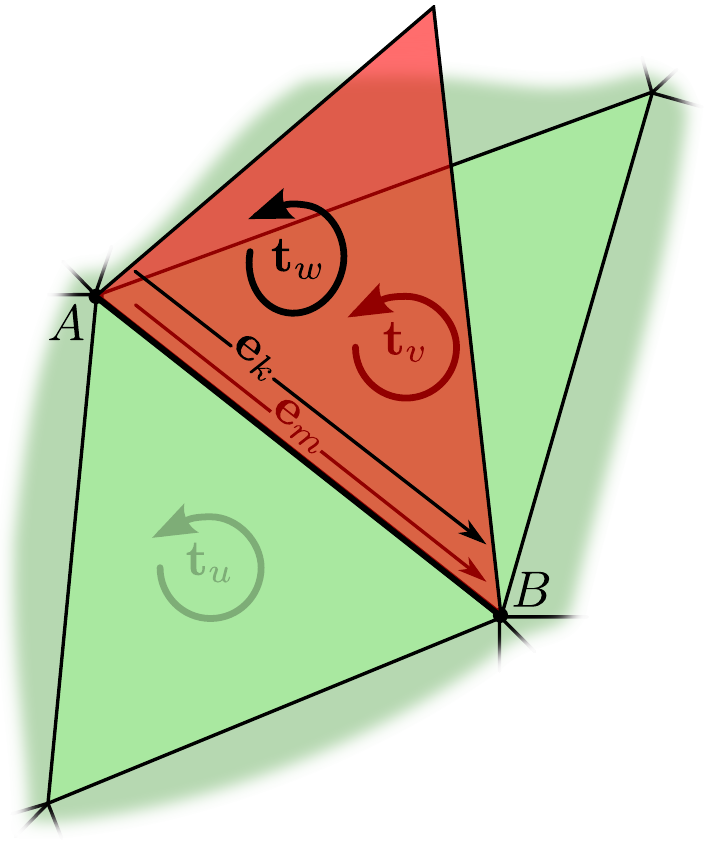
\includegraphics[width=\textwidth]{figures/badMesh3.png}
				\end{column}
				\begin{column}{.45\textwidth}
					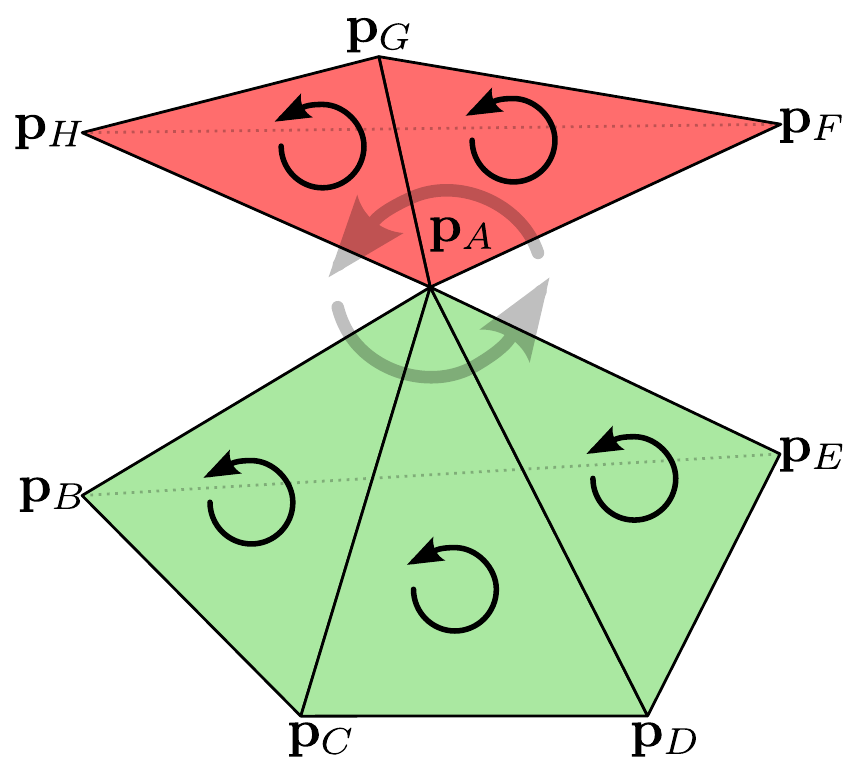
\includegraphics[width=\textwidth]{figures/badMesh1.png}
					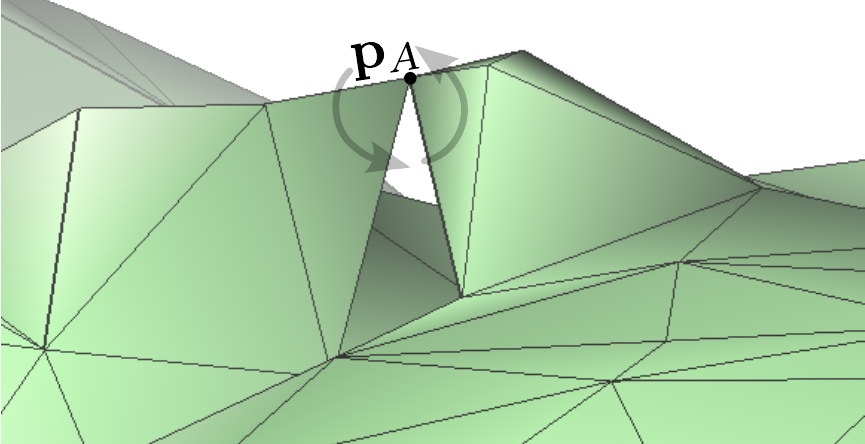
\includegraphics[width=\textwidth]{figures/badMesh2.png}
				\end{column}
			\end{columns}
		\end{column}
		\begin{column}{.475\textwidth}
			%\vspace*{4mm}
			\begin{itemize}
				\item Errors propagate in filter responses
				\item Jagged borders of segmented areas
			\end{itemize}
			\vspace*{4mm}
			\begin{columns}[T]
				\begin{column}{.1\textwidth}
				\end{column}
				\begin{column}{.45\textwidth}
					\centering
					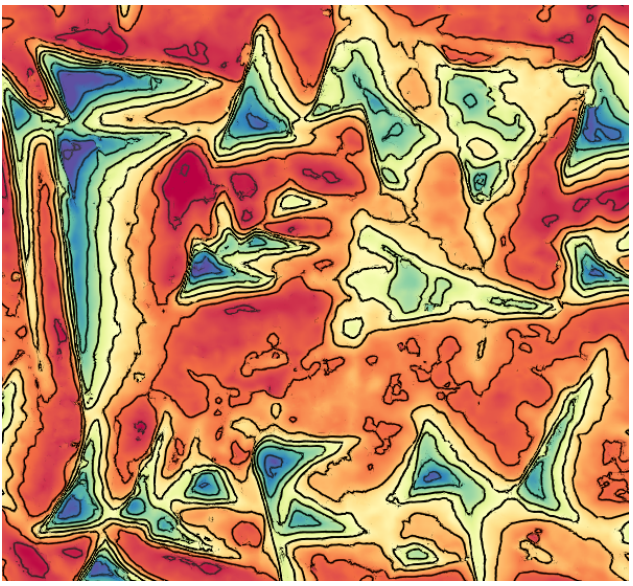
\includegraphics[width=\textwidth]{figures/beforeFilter.png}
					Before smoothing
				\end{column}
				\begin{column}{.45\textwidth}
					\centering
					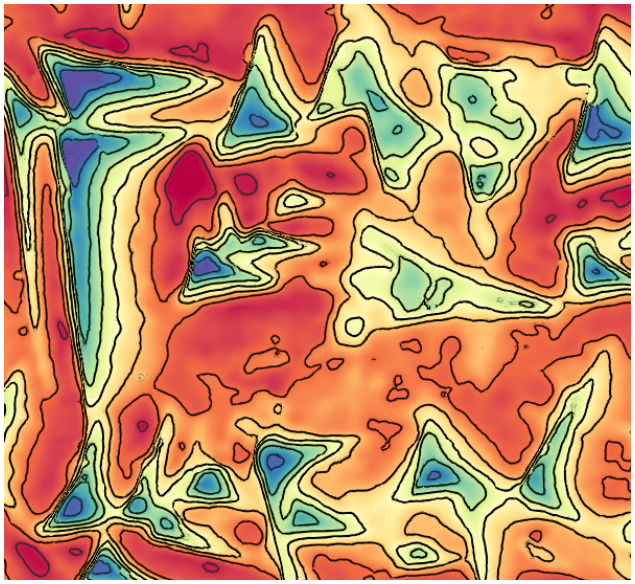
\includegraphics[width=\textwidth]{figures/afterFilter.png}
					After smoothing
				\end{column}
			\end{columns}
		\end{column}
	\end{columns}
}


%------------------------------------------------
\frame{\frametitle{Smoothing jagged borders of segmented areas}
	\vspace*{-4mm}
	\begin{columns}[T]
		\begin{column}{.5\textwidth}
			\centering
			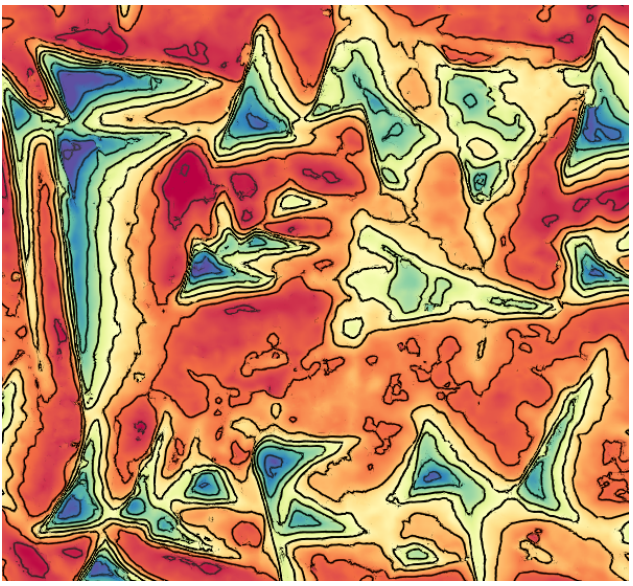
\includegraphics[width=.9\textwidth]{figures/beforeFilter.png}
			Before smoothing
		\end{column}
		\begin{column}{.5\textwidth}
			\centering
			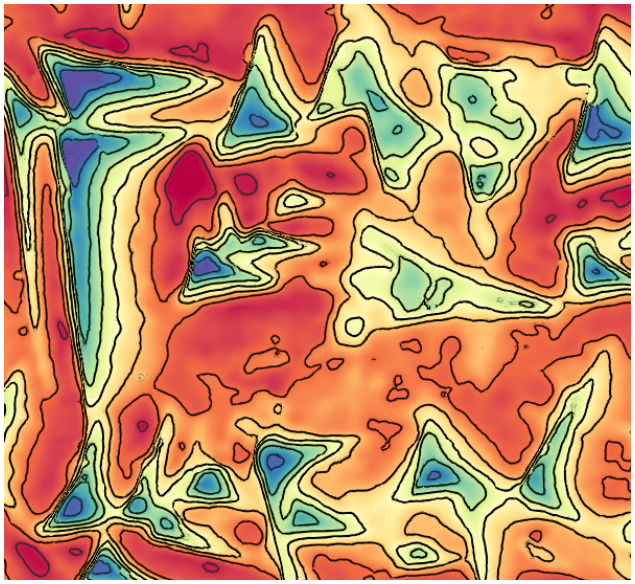
\includegraphics[width=.9\textwidth]{figures/afterFilter.png}
			After smoothing
		\end{column}
	\end{columns}
}

%------------------------------------------------
\frame{\frametitle{Increasing demand for high-definition, 3D~surface scans}
	\begin{columns}[T]
		\begin{column}{.45\textwidth}
			\begin{itemize}
				%\item Danger to physical archives
				\item Modernization of archeology
				\item High quality 3D-scanners are becoming less expensive
			\end{itemize}
		\end{column}
		\begin{column}{.55\textwidth}
			\centering
			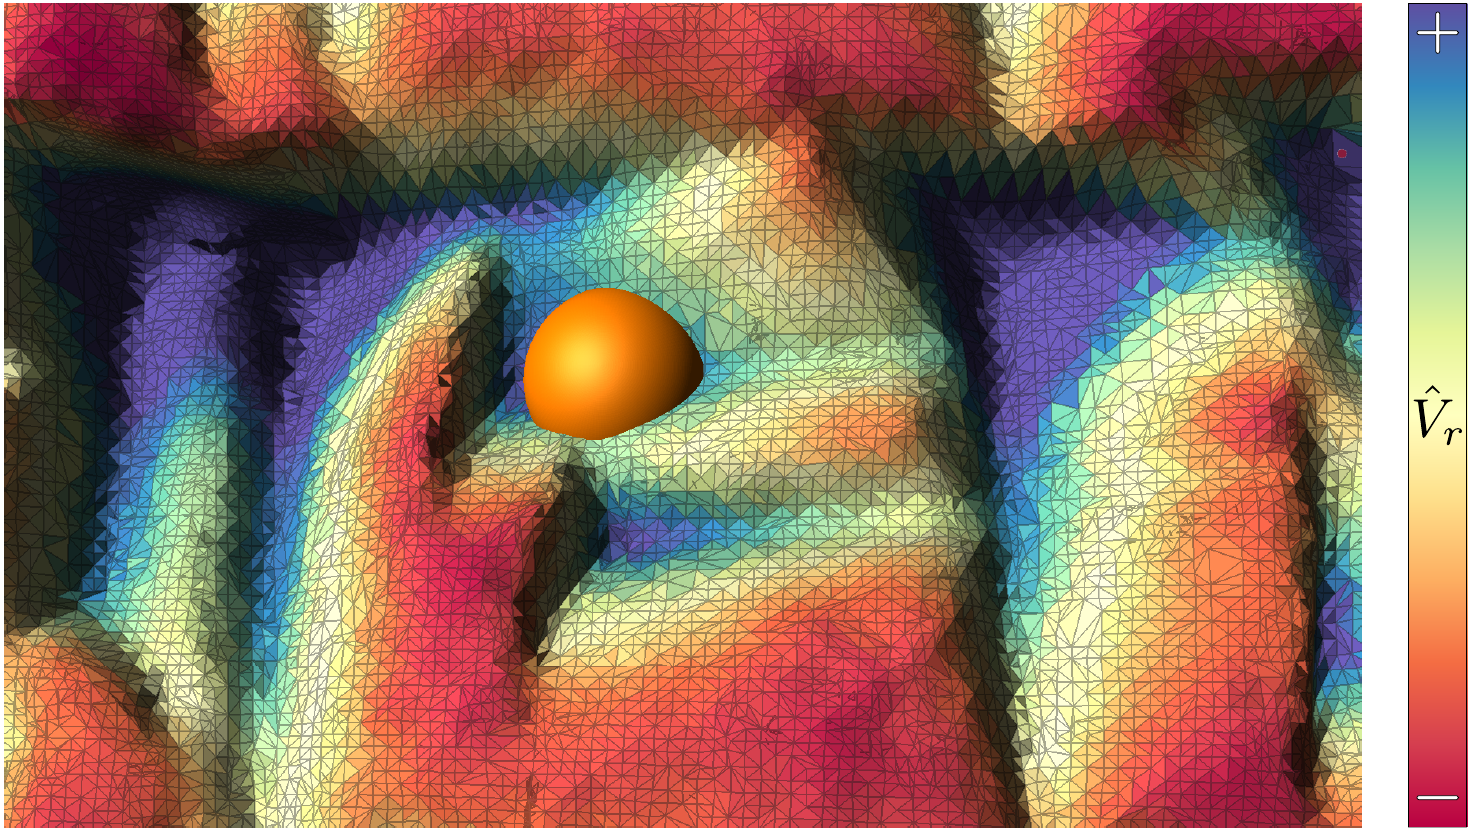
\includegraphics[width=1.0\linewidth]{figures/visualizeFunctionValues2.png}
			3D Surface Scan as a discrete 2D manifold \break colored by function value
		\end{column}
	\end{columns}
}

%------------------------------------------------
\frame{\frametitle{One-Ring Neighborhoods in Regular and Irregular Meshes}
	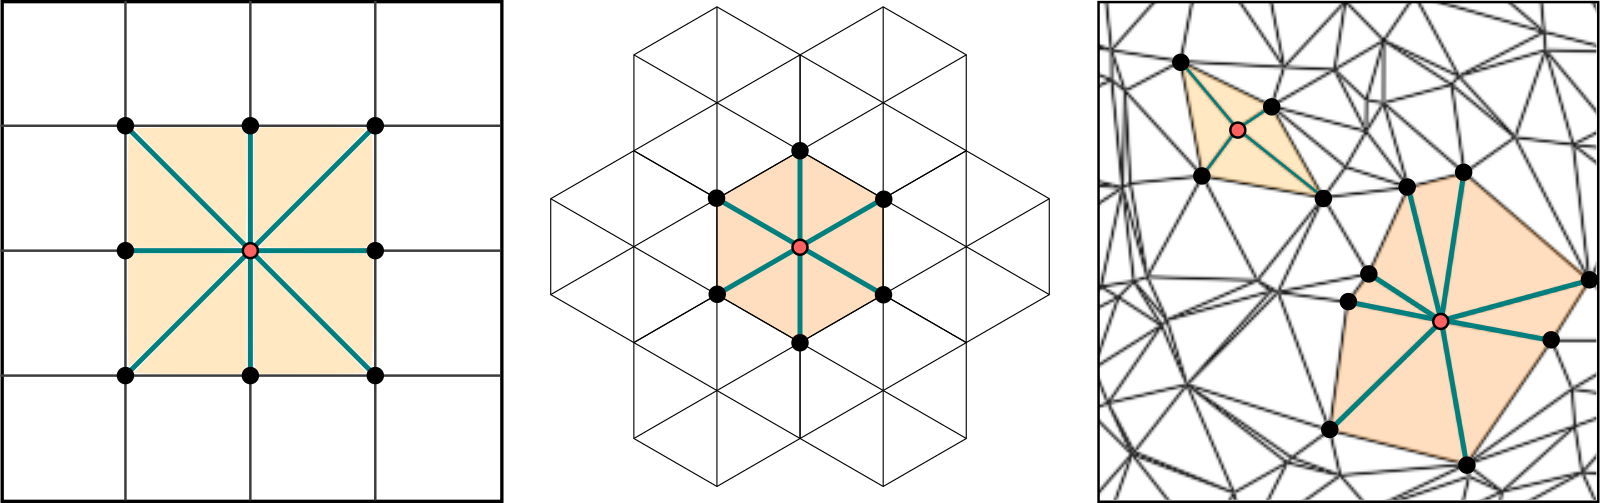
\includegraphics[width=1.0\linewidth]{figures/neighborhoods_presentation.png}

	\bigskip
	\begin{columns}[c]
		\begin{column}{.27\textwidth}
			a regular square mesh, as in pixels of a digital image
		\end{column}
		\begin{column}{.27\textwidth}
			a regular triangle mesh, as in a hexagonal tessellation
		\end{column}
		\begin{column}{.3\textwidth}
			an irregular triangle mesh, typical of acquired \tdd{}
		\end{column}
	\end{columns}
}

%------------------------------------------------
\frame{\frametitle{Anatomy of a Mesh}
	\begin{columns}[T]
		\begin{column}{.2\textwidth}
			\vspace*{-2mm}
			{\fontsize{10}{14}\selectfont
				\begin{tabular}{ l l }
					$\bP$ & the set of points \{$\bp_1$, \ldots, $\bp_n$\} \\
					$\bT$ & the set of triangle faces \{$\bt_1$, \ldots, $\bt_m$\} \\
					$\bF$ & the set of function values \{$f_1$, \ldots, $f_n$\} \\
					$\bM$ & the triangle mesh; a 2D discrete manifold \\
					~ & ~ \\
					$\bE$ & the set of lengths \{$\ell_{1,2}$, \ldots, $\ell_{n-1,n}$\} \\
					$\bN$ & the set of one-ring neighborhoods \\
					$\bN_2$ & the neighborhood of $\bp_2$
				\end{tabular}
			}
		\end{column}
		\begin{column}{.8\textwidth}
			\vspace*{2mm}
			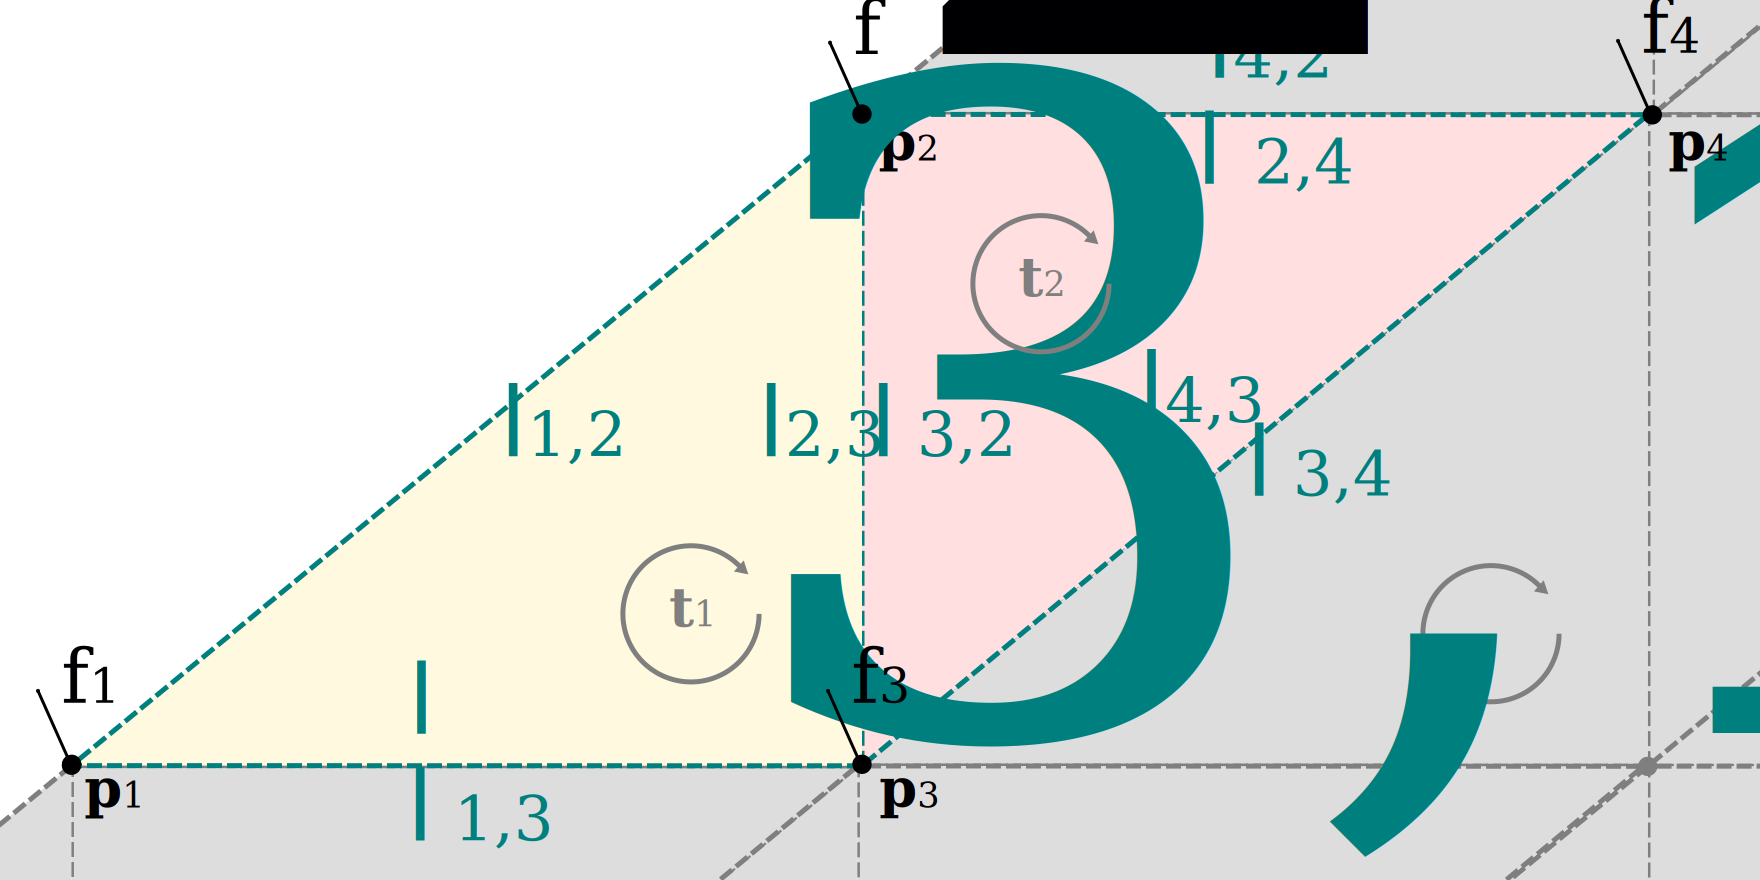
\includegraphics[width=\textwidth]{figures/triangularFaces_presentation.png}
		\end{column}
	\end{columns}
}




%================================================
%================================================
\section{Fast One-Ring Smoothing Filter}


%================================================
\subsection{Mathematical Foundation}

%------------------------------------------------
\frame{\frametitle{A One-Ring Neighborhood and its Geodesic Disc}
	\centering
	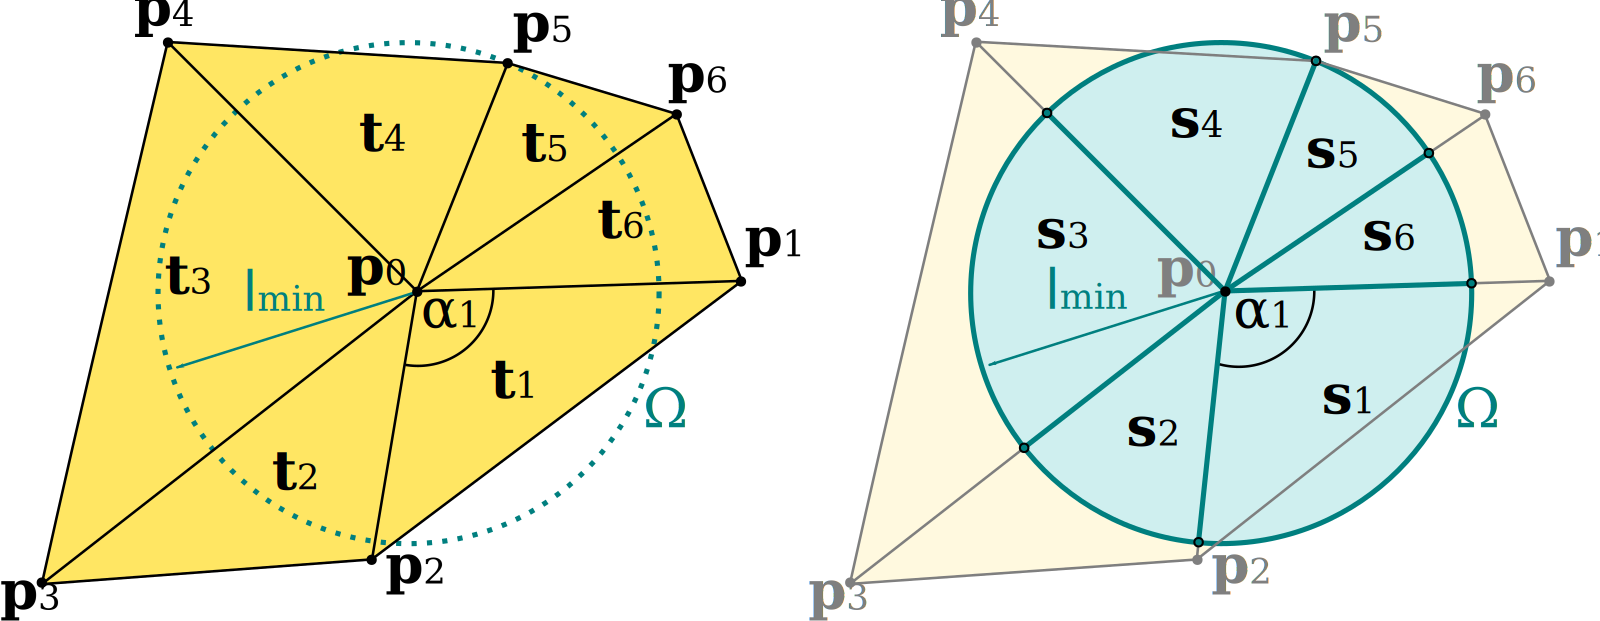
\includegraphics[width=0.8\linewidth]{figures/geodesicDisc_presentation.png}
	\begin{align*}
		{\color{MyTeal}\elm(\bp_0)}\; &{\color{black}:= \min_{\forall \bp_i \in \bN_v}|\bp_i - \bp_0|} \\
		{\color{MyTeal}\gelm}\; &{\color{black}:= \min\left \{{\color{MyTeal}\elm(\bp_0)} \;|\; \bp_0 \in \bM\,\right \}}
	\end{align*}
}

%------------------------------------------------
\frame{\frametitle{An Enhanced View of Circle Sector $\bs_1$}
	\vspace{-4mm}
	\begin{columns}[T]
		\begin{column}{.5\textwidth}
			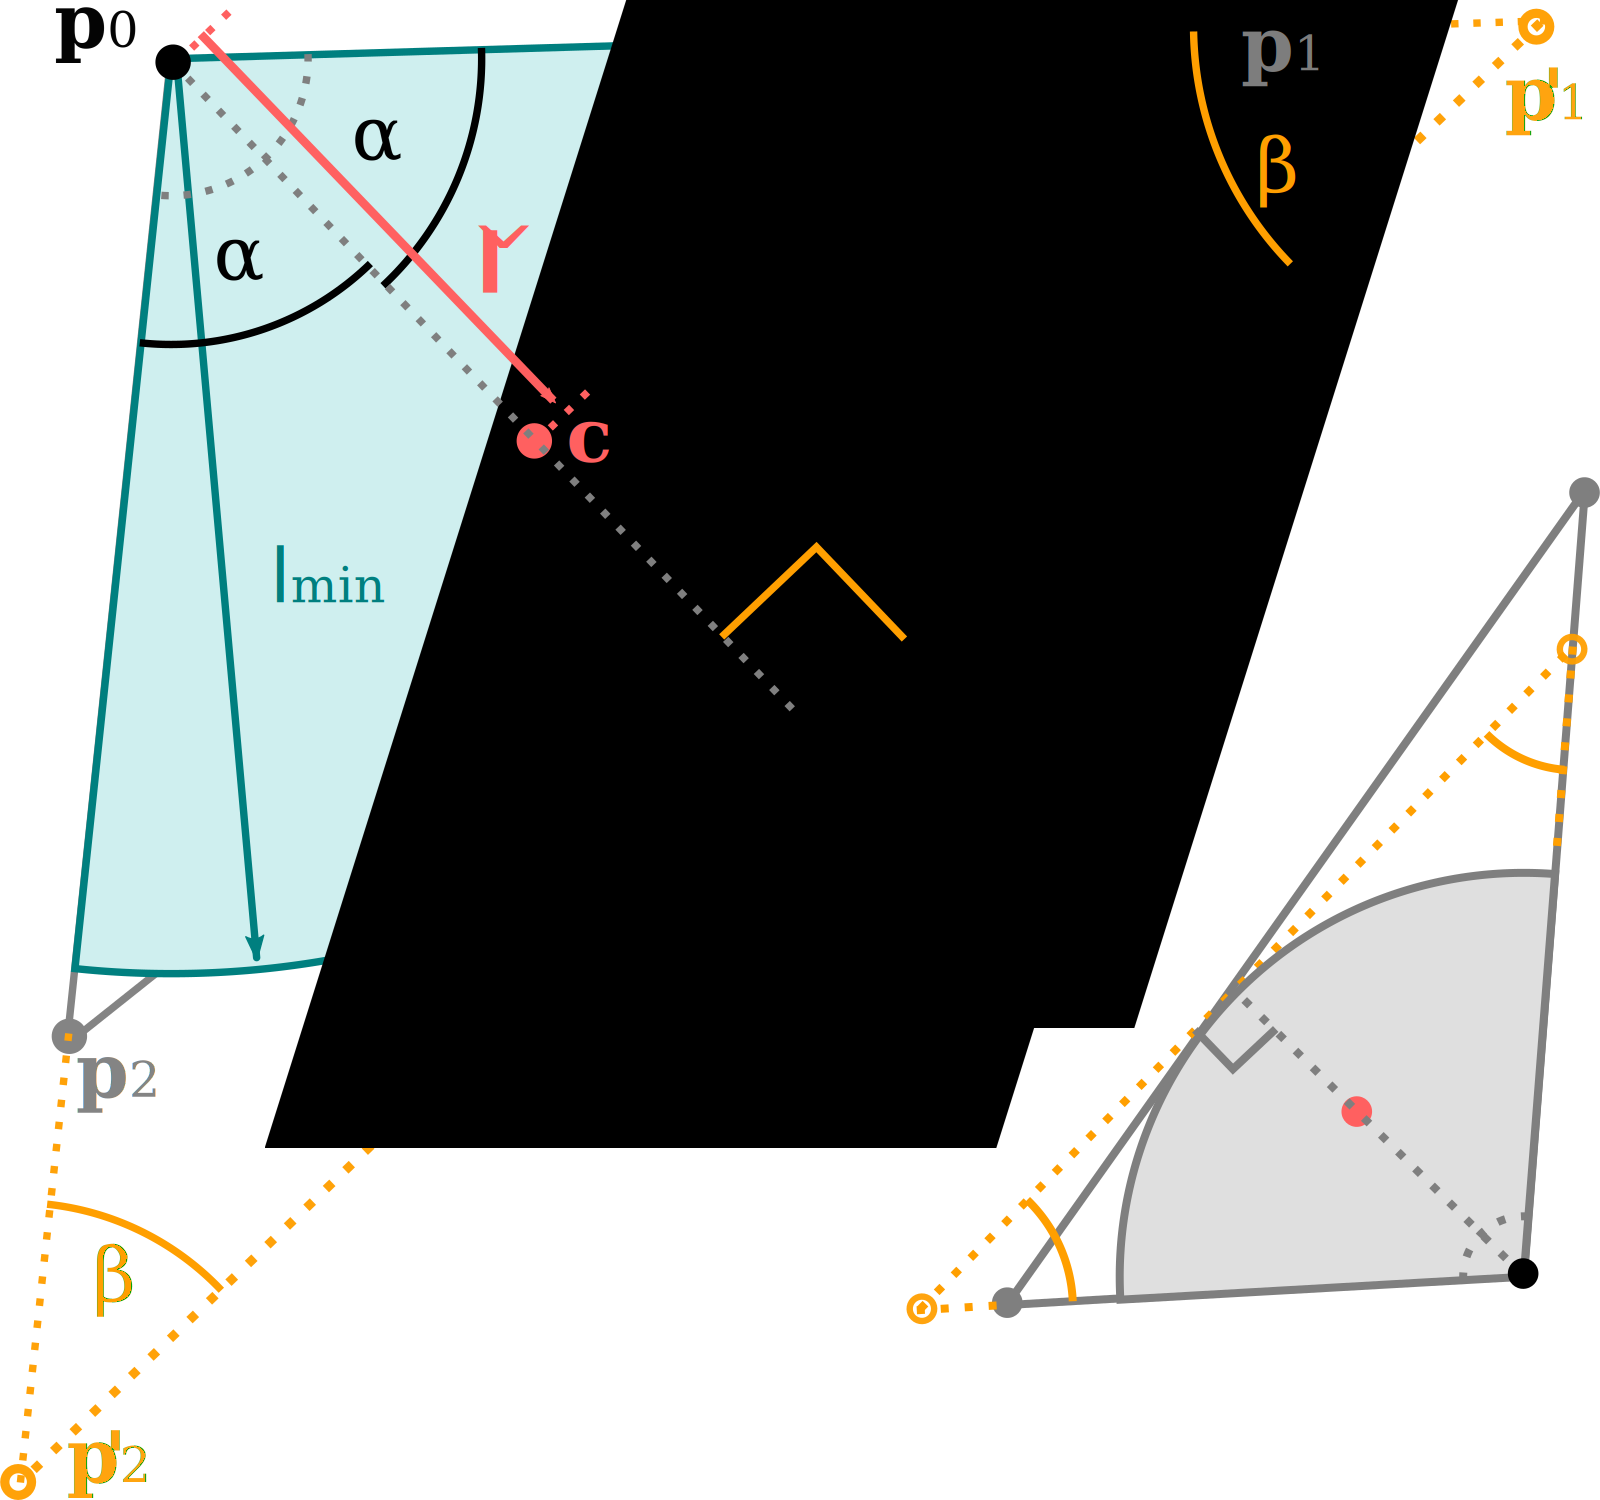
\includegraphics[width=\linewidth]{figures/anglesAndCenterOfGravity_presentation.png}
		\end{column}
		\begin{column}[t]{.5\textwidth}
			\begin{align*}
				{\color{black}\alpha}\; &{\color{black}:= cos^{-1}\left (\frac{\ell_{0,1}^2 + \ell_{0,2}^2 - \ell_{1,2}^2}{2\cdot\ell_{0,1}\cdot\ell_{0,2}}\right )} \\
				{\color{MySand}\beta}\; &{\color{MySand}:= \Big(\frac{\pi}{2} - \frac{{\color{black}\alpha}}{2}\Big) = \frac{(\pi - {\color{black}\alpha})}{2}} \\
				{\color{MyTeal}A}\; &{\color{MyTeal}:= \frac{\left (\,\gelm\,\right )^2{\color{black}\alpha}}{2}} \\
				%{\color{MySand}\tilde{\ell}_1}\; &{\color{MySand}:= \frac{{\color{MyTeal}\gelm}}{\lVert\bp_1 - \bp_0\lVert_2 \;\sin\left (\beta\right )}} \\
				{\color{MyCoral}\check{\ell}}\; &{\color{MyCoral}:= \frac{4\:{\color{MyTeal}\gelm}\:\sin(\frac{{\color{black}\alpha}}{2})}{3\,{\color{black}\alpha}}}
			\end{align*}
		\end{column}
	\end{columns}
}

%------------------------------------------------
\frame{\frametitle{Interpolation of function values to the center of gravity}
	\only<1>{
		\vspace*{-4mm}
		\begin{flushright}Load function values $f_0$, $f_1$, and $f_2$\end{flushright}
		\vspace*{-6mm}
		\centering
		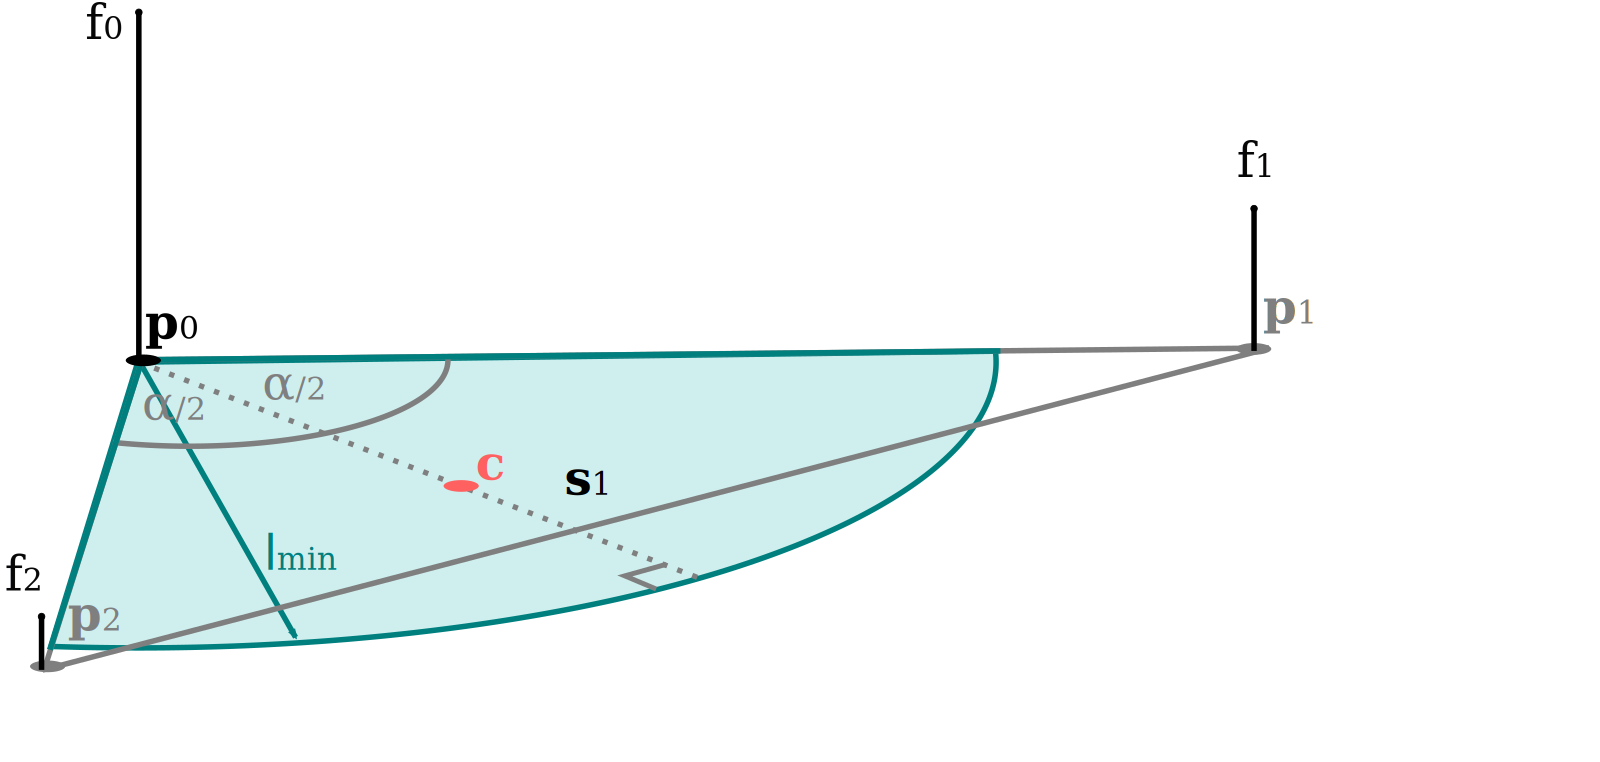
\includegraphics[width=0.95\linewidth]{figures/interpolatedFunctionValues_presentation1.png}
	}\only<2>{
		\vspace*{-4mm}
		\begin{flushright}Extrapolate $f_1$ and $f_2$ to circumscribing triangle\end{flushright}
		\vspace*{-6mm}
		\centering
		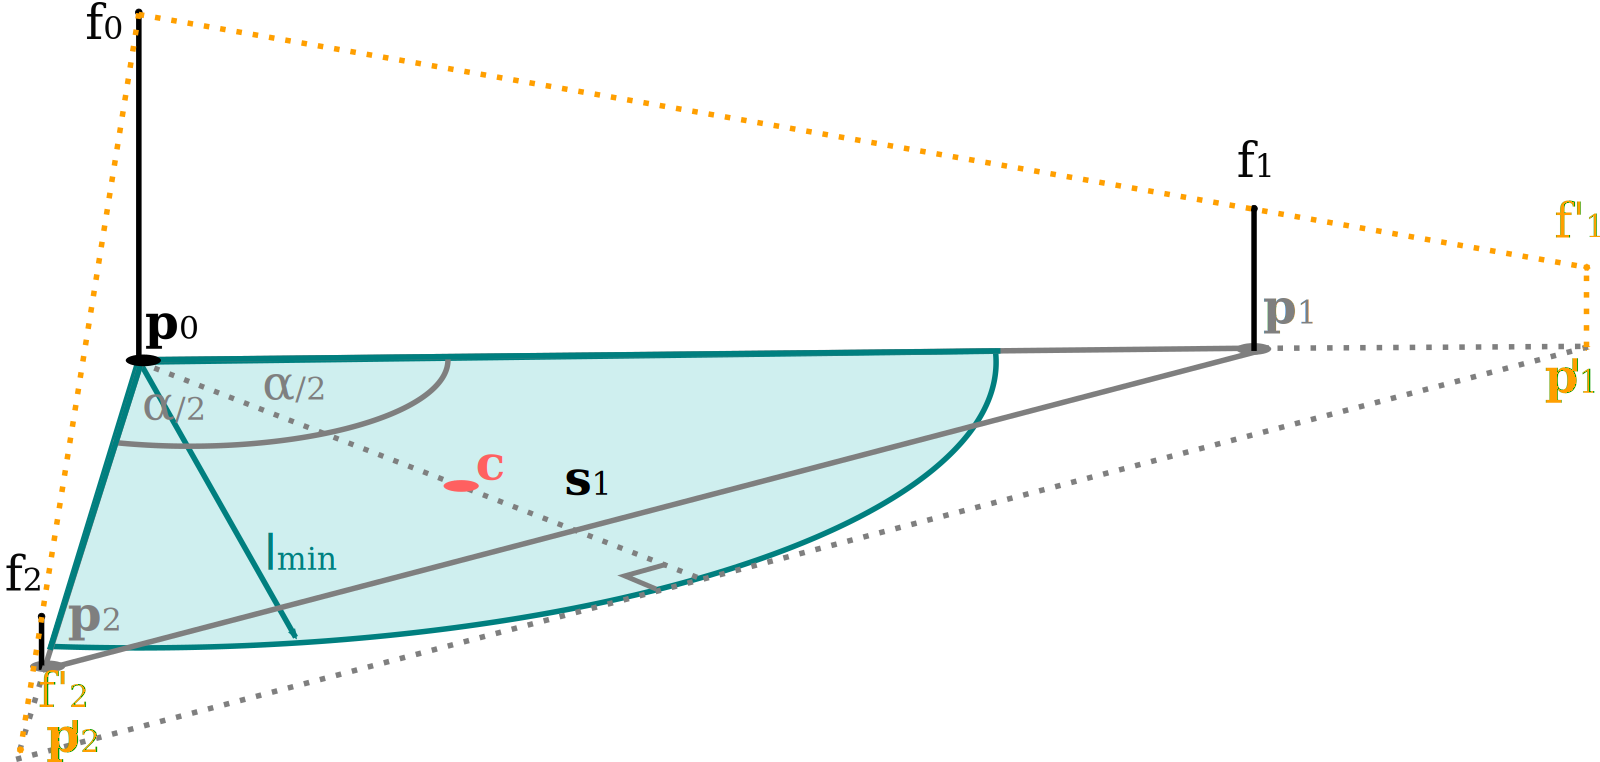
\includegraphics[width=0.95\linewidth]{figures/interpolatedFunctionValues_presentation2.png}
	}\only<3>{
		\vspace*{-4mm}
		\begin{flushright}Interpolate $f$'$_1$ and $f$'$_2$ to bisecting line\end{flushright}
		\vspace*{-6mm}
		\centering
		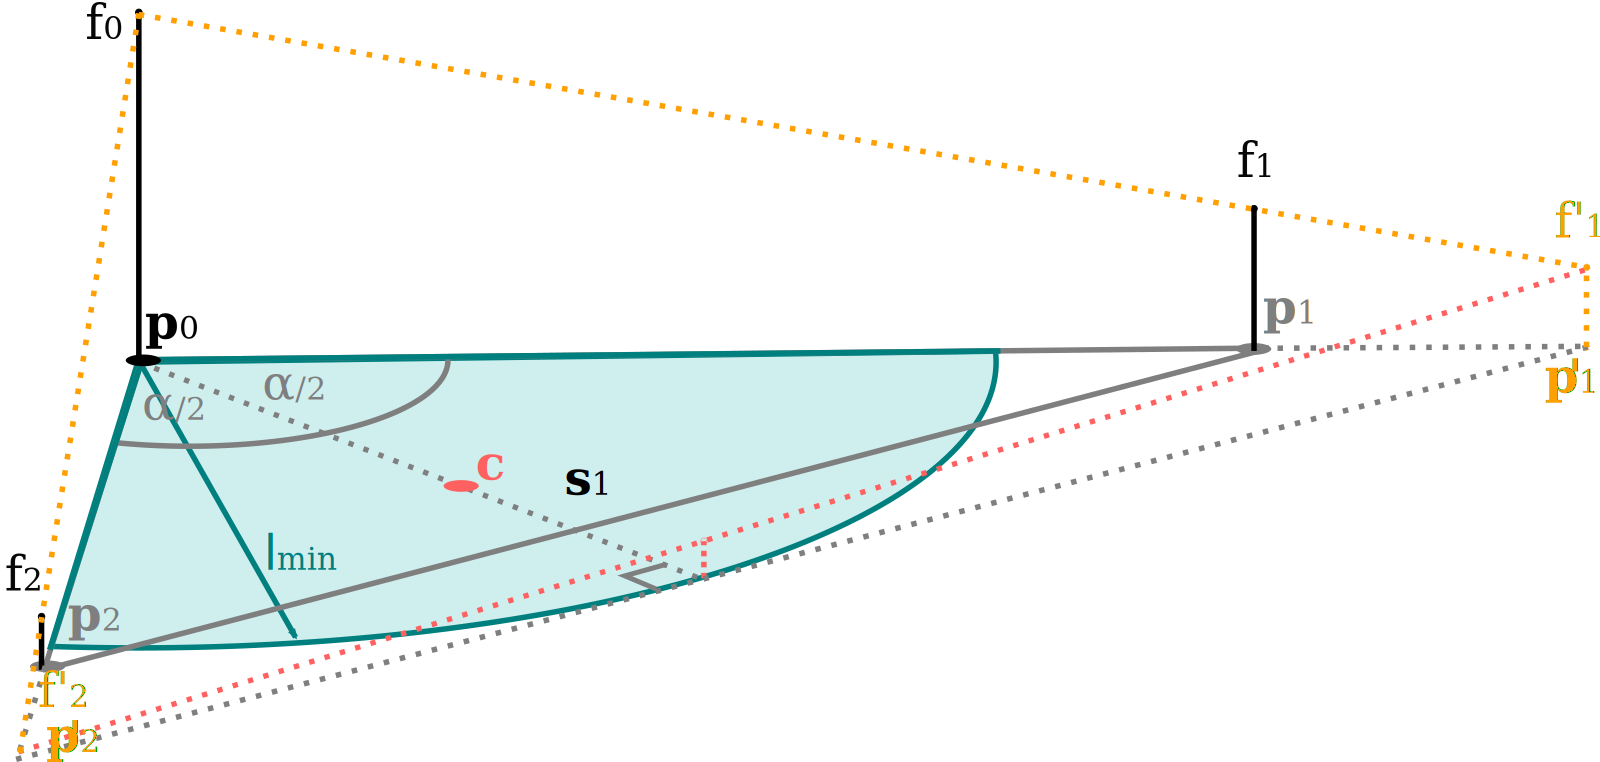
\includegraphics[width=0.95\linewidth]{figures/interpolatedFunctionValues_presentation3.png}
	}\only<4>{
		\vspace*{-4mm}
		\begin{flushright}Interpolate result and $f_0$ to center of gravity\end{flushright}
		\vspace*{-6mm}
		\centering
		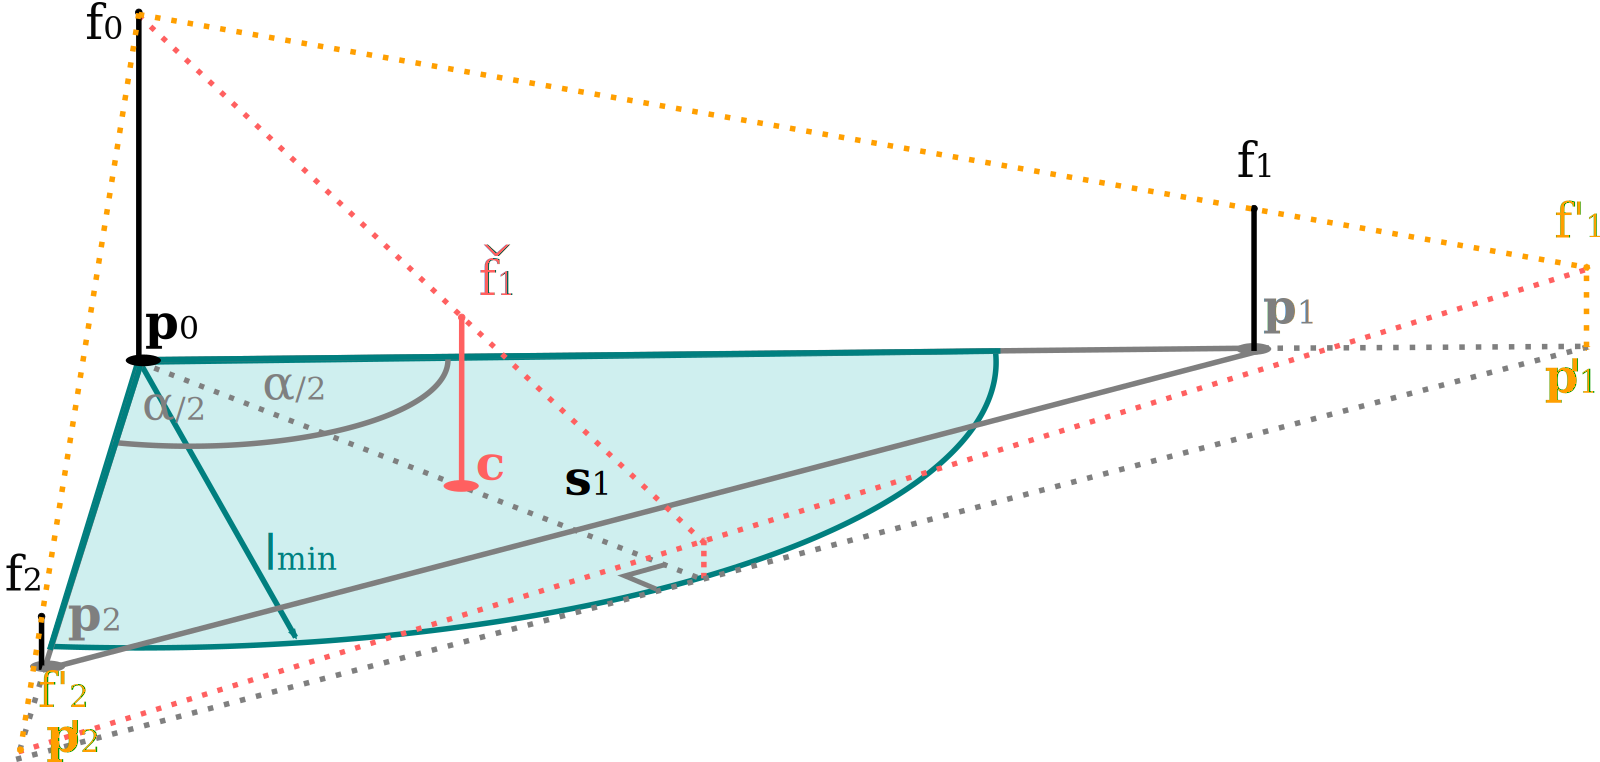
\includegraphics[width=0.95\linewidth]{figures/interpolatedFunctionValues_presentation4.png}
	}
}

%------------------------------------------------
%TODO: Fix bottom marigin
\frame{\frametitle{Filter Result - The weighted mean function value at $\bp_0$}
	\par \vspace*{-4mm}
	\begin{equation*}
		f'_0 := \frac{\sum A_i\check{f}_i}{\sum A_i} \quad \forall i \in \{1,\,\ldots,\,6\}
	\end{equation*}
	\vspace*{0mm}
	\centering
	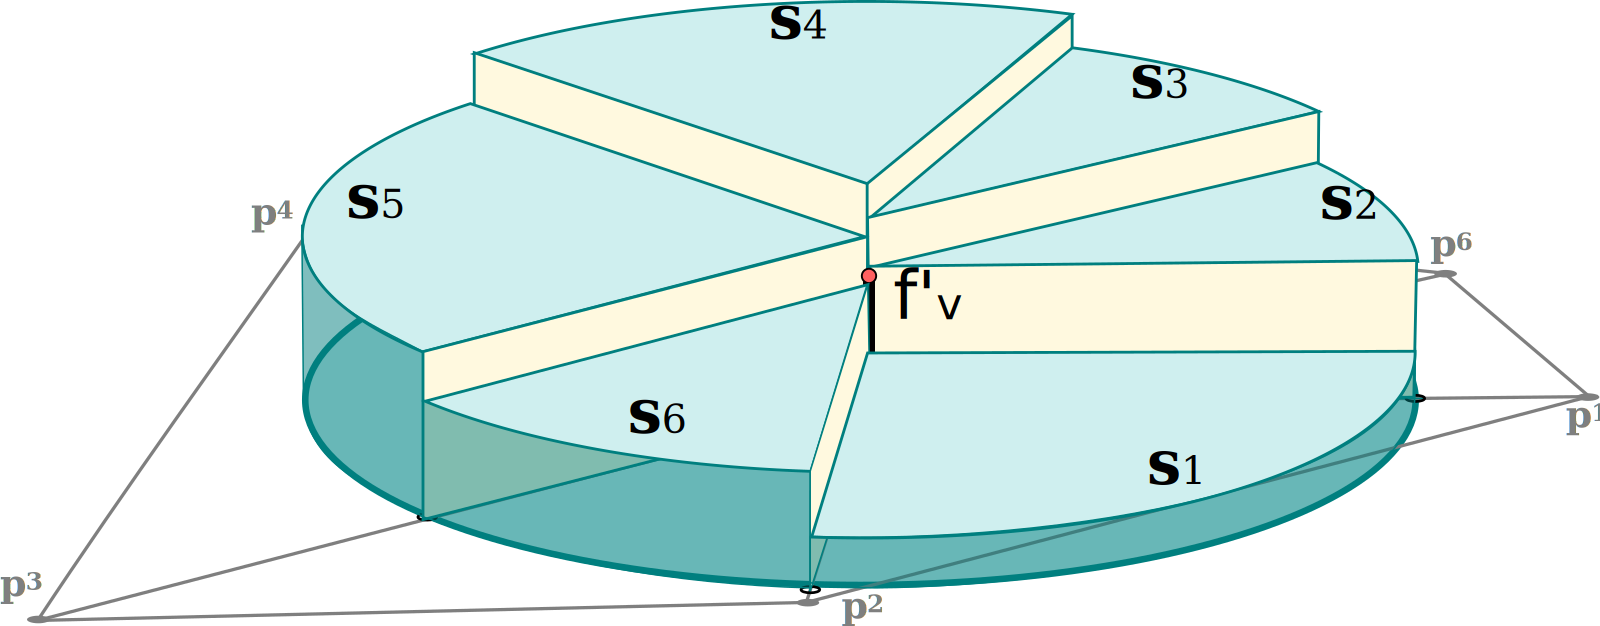
\includegraphics[width=1.0\linewidth]{figures/funcValVolumes_presentation.png}
}


%================================================
\subsection{Serial Algorithm}

%------------------------------------------------
%TODO: ADD nomenclature
\frame[c]{\frametitle{Serial Algorithm for Fast One-Ring Smoothing}
	\resizebox{1.0\textwidth}{!}{
		\begin{tikzpicture}[node distance=0cm]
			\node<1->(T)      [givNode, xshift=   0cm] {$\bT$};
			\node<1->(P)      [givNode, xshift=   0cm, yshift=-1.13cm] {$\bP$};
			\node<1->(bn)     [algNode, xshift= 3.0cm] {Build One-Ring \\ Neighborhoods};
			\node<1->(N)      [genNode, xshift= 6.0cm] {$\bN$};
			\node<2->(ce)     [algNode, xshift= 9.0cm, yshift=-2.81cm] {Calculate \\ Edge~Lengths};
			\node<3->(F)      [givNode, xshift=12.0cm] {$\bF$};
			\node<2->(E)      [genNode, xshift=12.0cm, yshift=-2.25cm] {$\bE$};
			\node<2->(gelm)   [genNode, xshift=12.0cm, yshift=-3.38cm] {$\gelm$};
			\node<3->(cf)     [algNode, xshift=15.0cm, yshift=-1.13cm] {Convolve \\ Filter};
			\node<3->(Fprime) [outNode, xshift=18.0cm, yshift=-1.13cm] {$\bF'$};

			\node<1->(empty)  [minimum width=1cm, xshift=18.0cm] {\null};
			\node<1->(empty)  [minimum height=1cm, yshift=-3.38cm] {\null};

			\draw<1->[->, givLine] (T) -- (bn);
			\draw<1->[->, givLine] (P) -- (bn);
			\draw<1->[->, algLine] (bn) -- (N);
			\draw<2->[->, genLine] (N) -- (ce);
			\draw<2->[->, givLine] (P) -- (ce);
			\draw<2->[->, algLine] (ce) -- (E);
			\draw<2->[->, algLine] (ce) -- (gelm);
			\draw<3->[->, givLine] (F) -- (cf);
			\draw<3->[->, genLine] (N) -- (cf);
			\draw<3->[->, genLine] (E) -- (cf);
			\draw<3->[->, genLine] (gelm) -- (cf);
			\draw<3->[->, givLine] (P) .. controls (6cm,-1.25cm) .. (cf.185);
			\draw<3->[->, algLine] (cf) -- (Fprime);
			\draw<4->[->, outLine] (Fprime.north) .. controls (18cm,0cm) .. (15.0cm,0cm)
				node[tealStyle, rounded corners, yshift=.1cm]{$\tau$ iterations} -- (F);
		\end{tikzpicture}
	}
}

%------------------------------------------------
\frame{\frametitle{Towards Acceleration}
	\centering
	{\Huge Unfortunately, this is very slow!}

	\medskip
	\scalebox{-1}[1]{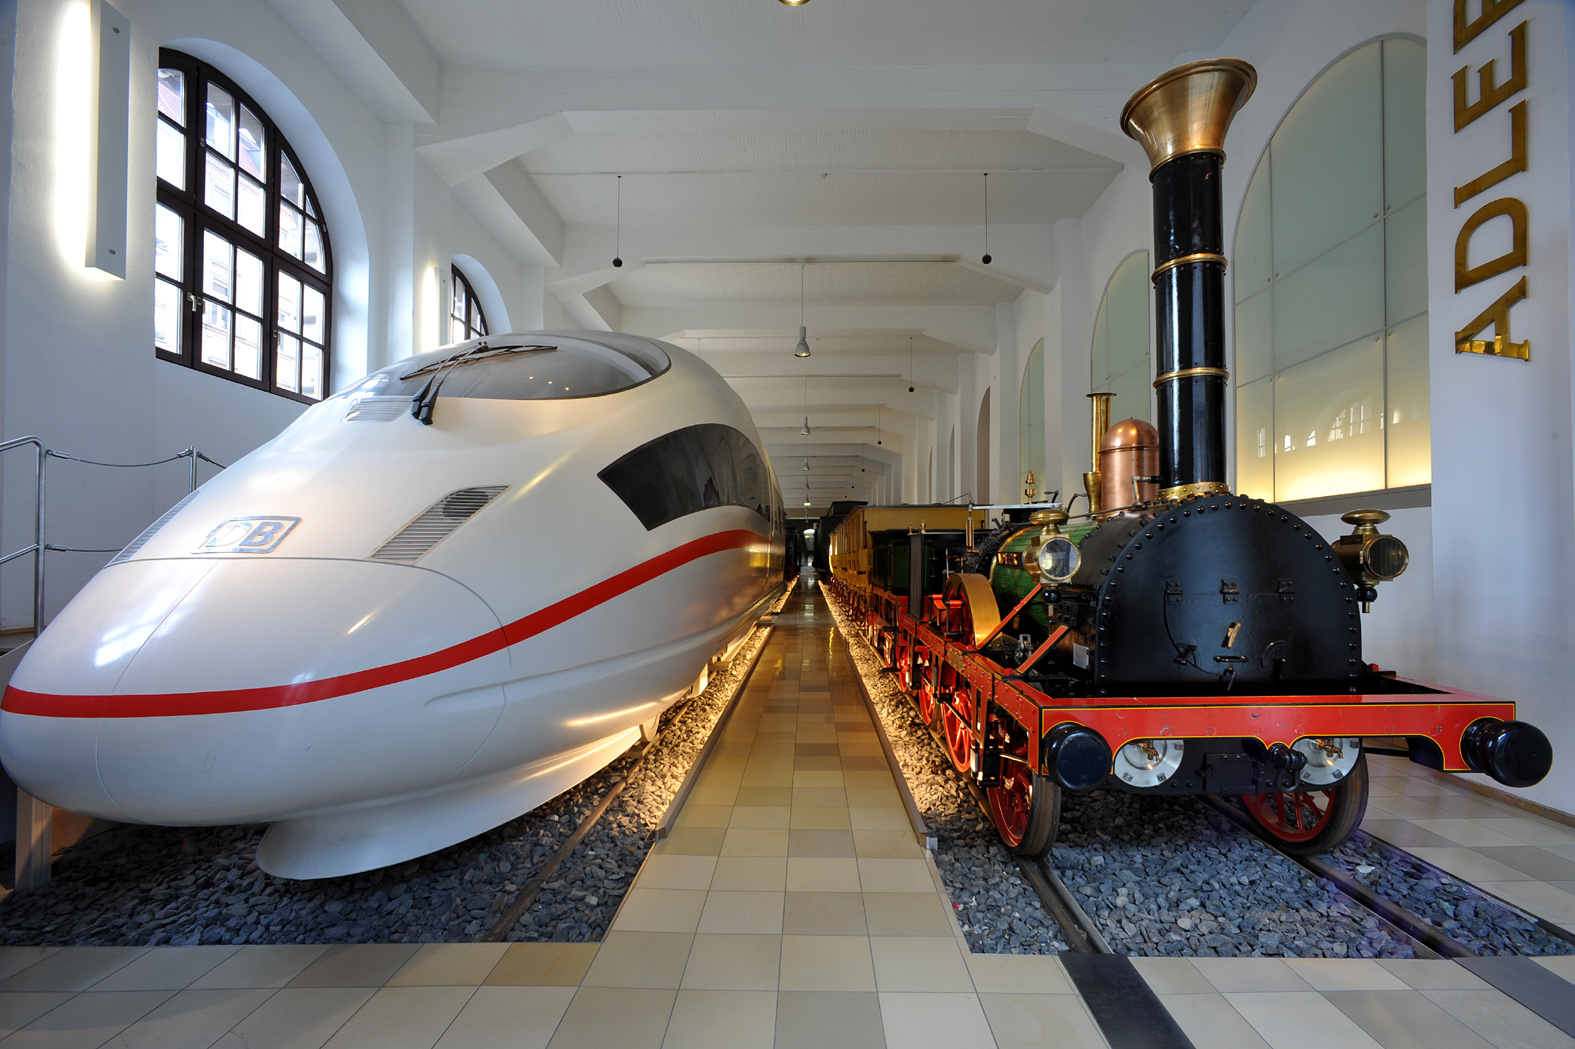
\includegraphics[width=0.5\linewidth]{figures/DB_Museum_Nuernberg.jpg}}

	\medskip
	...thankfully, a modern solution exists.
}




%================================================
%================================================
\section{Exploiting Parallelism}


%================================================
\subsection{Some Basics}

%------------------------------------------------
\frame{\frametitle{SIMD Architecture (Single Instruction, Multiple Data)}
	\vspace*{4mm}
	\includegraphics[width=1.0\linewidth]{figures/tikz/simdArchitecture.pdf}

	\bigskip
	\begin{flushright}
		i.e. Supercomputers, GPGPUs, Computer Pools %Name examples like the cray, and pool in this building
	\end{flushright}
}

%------------------------------------------------
\frame{\frametitle{CPU vs GPU Construction}
	\centering
	ALU (Arithmatic \& Logic Unit) aka. ``compute core'' \par
	\vspace*{4mm}
	\includegraphics[width=1.0\linewidth]{figures/cpuvgpu.png}
}

%------------------------------------------------
\frame{\frametitle{Amdahl's law and the Degree of Parallelism}
	\begin{columns}[T]
		\begin{column}{.48\textwidth}
			Degree of Parallelism: the maximum share of operations that can be executed in parallel

			\medskip
			\begin{block}{Amdahl's law}
				Given a constant problem size $\hat{n}_{fixed}$,
				\begin{equation*}
					\lim_{\rho \to \infty} \mathit{S}(\hat{n}_{fixed},\,\rho) = 1 / q
				\end{equation*}
			\end{block}

			\medskip
			\textbf{Conclusion}: one \emph{cannot} simply add more processors in order to gain appreciable speedup!
		\end{column}
		\begin{column}{.52\textwidth}
			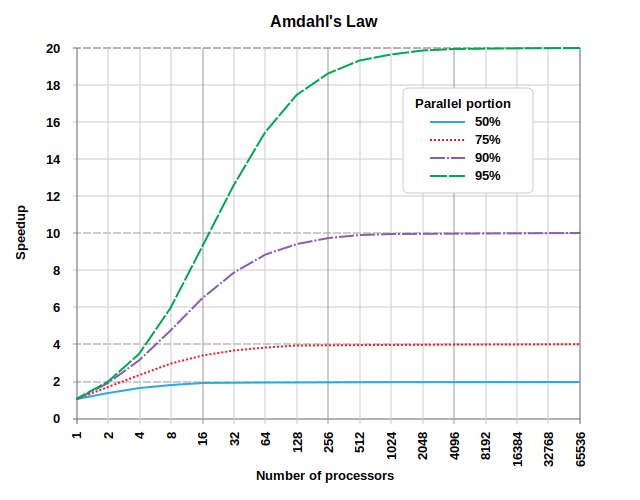
\includegraphics[width=1.1\textwidth]{figures/amdahlsLaw.png}
		\end{column}
	\end{columns}
}


%================================================
\subsection{Data Dependencies}

%------------------------------------------------
\frame{\frametitle{Data Dependencies in Serial Algorithm Build Neighborhoods}
	\centering
	\includestandalone[width=0.725\textwidth]{figures/tikz/sabnDataDependencies}
}

%------------------------------------------------
\frame{\frametitle{Data Dependencies in Serial Algorithm Calculate Edge Lengths}
	\centering
	\includestandalone[width=0.875\textwidth]{figures/tikz/sacelDataDependencies}
}

%------------------------------------------------
\frame{\frametitle{Data Dependencies in Serial Algorithm Convolve Filter}
	\only<1>{
		\centering
		\includestandalone[width=0.4825\textwidth]{figures/tikz/sacfDataDependencies}
	}\only<2>{
		\begin{columns}
			\begin{column}{.25\textwidth}
				\hspace*{-30mm}
				\includestandalone[width=1.93\textwidth]{figures/tikz/sacfDataDependencies}
			\end{column}
			\begin{column}{.75\textwidth}
				\centering
				\includestandalone[width=0.6\textwidth]{figures/tikz/sacfDataDependencies_excerpt}
			\end{column}
		\end{columns}
	}
	\begin{tikzpicture}[overlay, remember picture]
		\draw<2>[black,ultra thick,rounded corners] (6mm, 70mm) rectangle (36mm, 19mm);
		\draw<2>[gray,dotted,ultra thick] (36mm, 70mm) -- (60mm, 71mm);
		\draw<2>[gray,dotted,ultra thick] (36mm, 19mm) -- (60mm, 10mm);
	\end{tikzpicture}
}


%================================================
\subsection{Parallel Algorithm}

%------------------------------------------------
%TODO: ADD nomenclature
\frame[c]{\frametitle{Parallel Algorithm for Fast One-Ring Smoothing}
	\resizebox{1.0\textwidth}{!}{
		\begin{tikzpicture}[node distance=0cm]
			\node<1->(T)      [givNode, xshift= 0cm] {$\bT$};
			\node<1->(P)      [givNode, xshift= 0cm, yshift=-1.13cm] {$\bP$};
			\node<1->(rho)    [givNode, xshift= 0cm, yshift=-2.25cm] {$\rho$};
			\node<1->(bn)     [algNode, xshift= 3cm] {Build \\ Neighborhoods};
			\node<1->(N)      [genNode, xshift= 6cm] {$\bN$};
			\node<2->(cn)     [algNode, xshift= 9cm, yshift= 1.13cm] {Census \\ Neighborhoods};
			\node<2->(hatn)   [genNode, xshift=12cm, yshift= 1.13cm] {$\hat{n}$};
			\node<3->(ce)     [algNode, xshift=15cm, yshift=-2.81cm] {Calculate \\ Edge~Lengths};
			\node<3->(E)      [genNode, xshift=18cm, yshift=-2.25cm] {$\bE$};
			\node<3->(gelm)   [genNode, xshift=18cm, yshift=-3.38cm] {$\gelm$};
			\node<4->(F)      [givNode, xshift=18cm, yshift= 1.13cm] {$\bF$};
			\node<4->(cf)     [algNode, xshift=21cm, yshift=-1.13cm] {Convolve \\ Filter};
			\node<4->(Fprime) [outNode, xshift=24cm, yshift=-1.13cm] {$\bF'$};
			\node<1->(empty)  [minimum width=1cm, xshift=24cm] {\null};
			\node<1->(empty)  [minimum height=1cm, yshift=-3.38cm] {\null};
			\node<1->(empty)  [minimum height=1.75cm, yshift= 1.13cm] {\null};

			\draw<1->[->, givLine] (rho) .. controls (3cm,-2.25cm) .. (bn);
			\draw<1->[->, givLine] (T) -- (bn);
			\draw<1->[->, givLine] (P) -- (bn);
			\draw<1->[->, algLine] (bn) -- (N);
			\draw<2->[->, givLine] (rho) .. controls (6cm,-2.25cm) .. (cn);
			\draw<2->[->, genLine] (N) -- (cn);
			\draw<2->[->, algLine] (cn) -- (hatn);
			\draw<3->[->, givLine] (rho) .. controls (12cm,-2.25cm) and (6cm,-2.81cm) .. (ce);
			\draw<3->[->, givLine] (P) -- (ce);
			\draw<3->[->, genLine] (N) -- (ce);
			\draw<3->[->, genLine] (hatn) -- (ce);
			\draw<3->[->, algLine] (ce) -- (E);
			\draw<3->[->, algLine] (ce) -- (gelm);
			\draw<4->[->, givLine] (rho) .. controls (15cm,-2.25cm) and (9cm,-1.13cm) .. (cf.190);
			\draw<4->[->, givLine] (P) -- (cf);
			\draw<4->[->, genLine] (N) -- (cf);
			\draw<4->[->, genLine] (hatn) -- (cf);
			\draw<4->[->, genLine] (E) -- (cf);
			\draw<4->[->, genLine] (gelm) -- (cf);
			\draw<4->[->, givLine] (F) -- (cf);
			\draw<4->[->, algLine] (cf) -- (Fprime);
			\draw<5->[->, outLine] (Fprime.north) .. controls (24cm,1.13cm) .. (21.0cm,1.13cm)
				node[tealStyle, rounded corners, yshift=.1cm]{$\tau$ iterations} -- (F);
		\end{tikzpicture}
	}
}




%================================================
%================================================
\section{Experiments \& Evaluation}


%================================================
%TODO: Widen space between images
\subsection{Filter Response on Synthetic and Acquired Data}

%------------------------------------------------
\frame{\frametitle{Quadrisected-Square Tessellations}
	\vspace*{-3mm}
	\begin{columns}
		\begin{column}{0.17\textwidth}~\end{column}
		\begin{column}{0.22\textwidth}
			\centering
			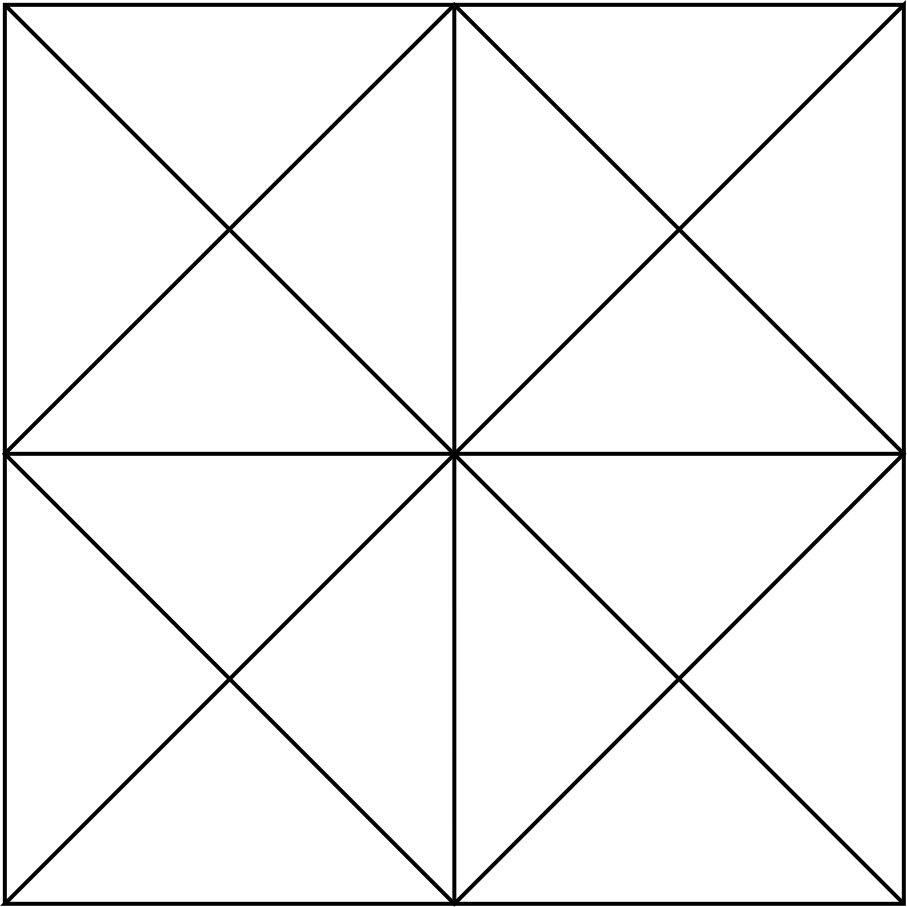
\includegraphics[width=.85\textwidth]{data/synthetic_meshes/square_tesselation_4tri_Dirac_delta_1_v13_f16_wireframe.png}
			{\footnotesize
				\par \vspace{-1mm} $r=1$,
				\par \vspace{-1mm} wireframe
			}
		\end{column}
		\begin{column}{0.22\textwidth}
			\centering
			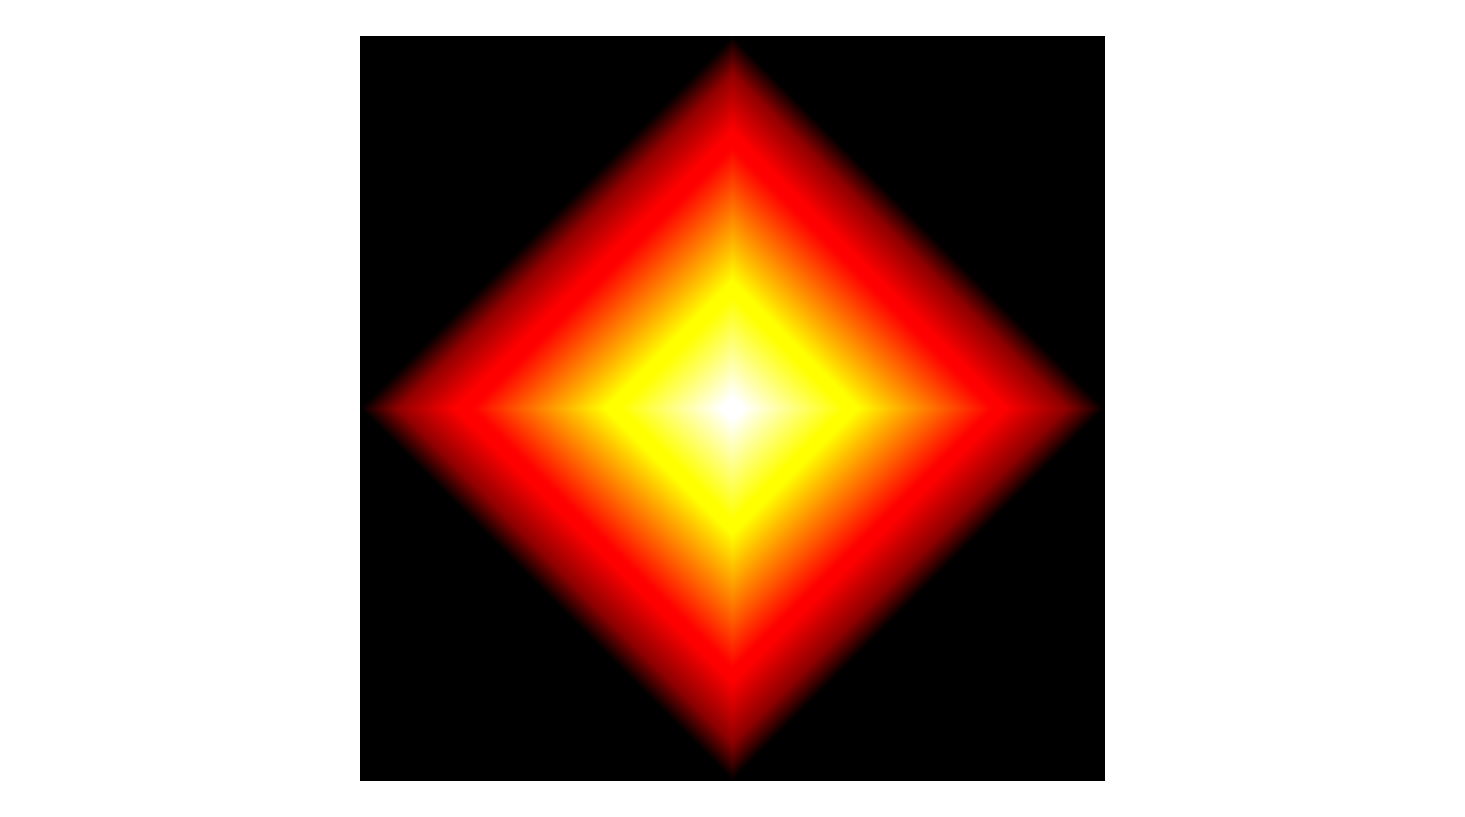
\includegraphics[width=.85\textwidth]{data/synthetic_meshes/square_tesselation_4tri_Dirac_delta_1_v13_f16_funcvals_0iter.png}
			{\footnotesize
				\par \vspace{-1mm} $r=1$,
				\par \vspace{-1mm} $0$~iterations
			}
		\end{column}
		\begin{column}{0.22\textwidth}
			\centering
			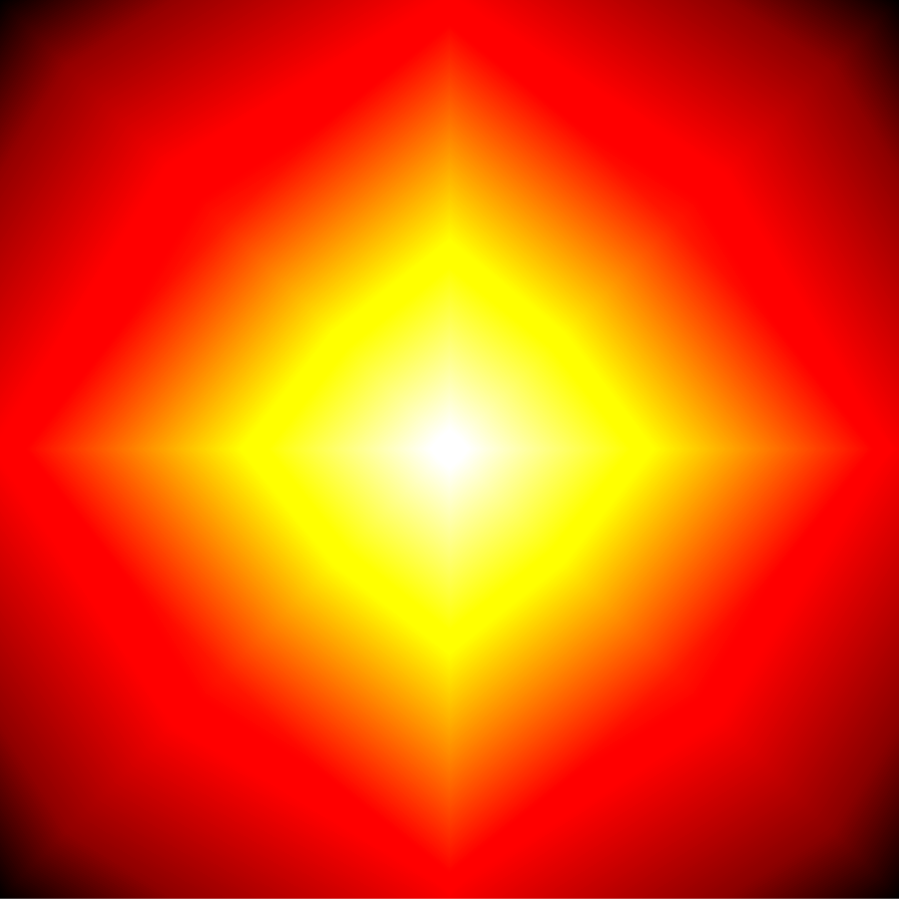
\includegraphics[width=.85\textwidth]{data/synthetic_meshes/square_tesselation_4tri_Dirac_delta_1_v13_f16_funcvals_1iter.png}
			{\footnotesize
				\par \vspace{-1mm} $r=1$,
				\par \vspace{-1mm} $1$~iteration
			}
		\end{column}
		\begin{column}{0.17\textwidth}~\end{column}
	\end{columns}
	\vspace*{4mm}
	\begin{columns}
		\begin{column}{0.17\textwidth}~\end{column}
		\begin{column}{0.22\textwidth}
			\centering
			
\includegraphics[width=.85\textwidth]{data/synthetic_meshes/square_tesselation_4tri_Dirac_delta_10_v841_f1600_wireframe_2.png}
			{\footnotesize
				\par \vspace{-1mm} $r=10$,
				\par \vspace{-1mm} wireframe
			}
		\end{column}
		\begin{column}{0.22\textwidth}
			\centering
			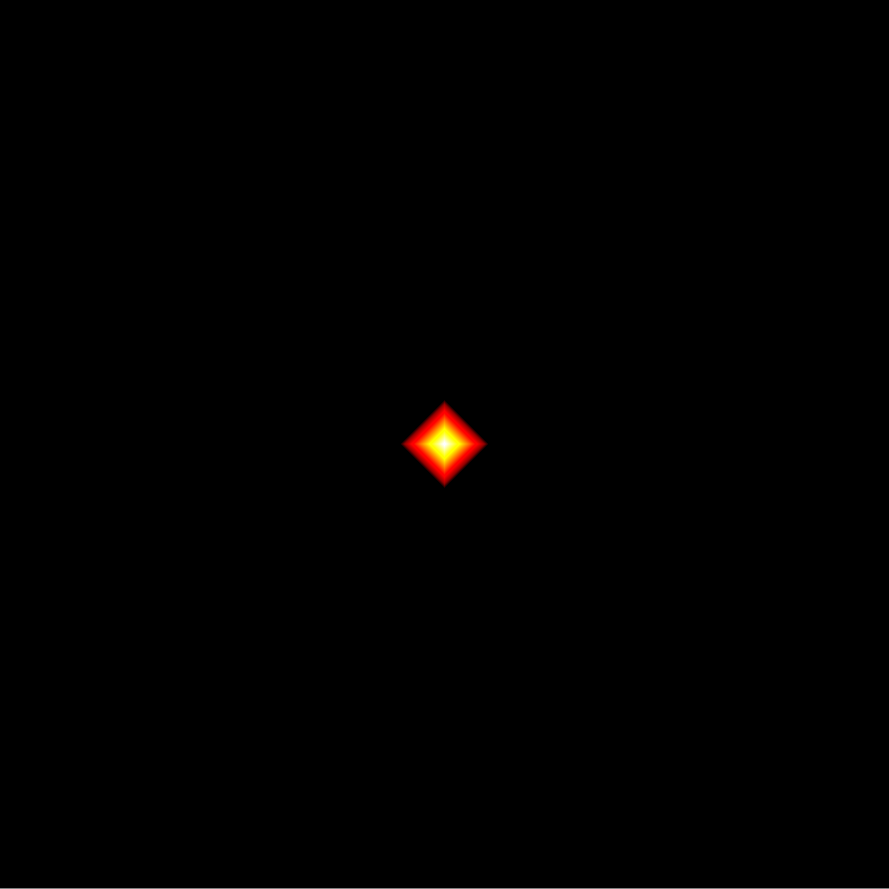
\includegraphics[width=.85\textwidth]{data/synthetic_meshes/square_tesselation_4tri_Dirac_delta_10_v841_f1600_funcvals_0iter.png}
			{\footnotesize
				\par \vspace{-1mm} $r=10$,
				\par \vspace{-1mm} $0$~iterations
			}
		\end{column}
		\begin{column}{0.22\textwidth}
			\centering
			
\includegraphics[width=.85\textwidth]{data/synthetic_meshes/square_tesselation_4tri_Dirac_delta_10_v841_f1600_funcvals_100iter.png}
			{\footnotesize
				\par \vspace{-1mm} $r=10$,
				\par \vspace{-1mm} $100$~iterations
			}
		\end{column}
		\begin{column}{0.17\textwidth}~\end{column}
	\end{columns}
}

%------------------------------------------------
\frame{\frametitle{Bisected-Square Tessellations}
	\vspace*{-3mm}
	\begin{columns}
		\begin{column}{0.17\textwidth}~\end{column}
		\begin{column}{0.22\textwidth}
			\centering
			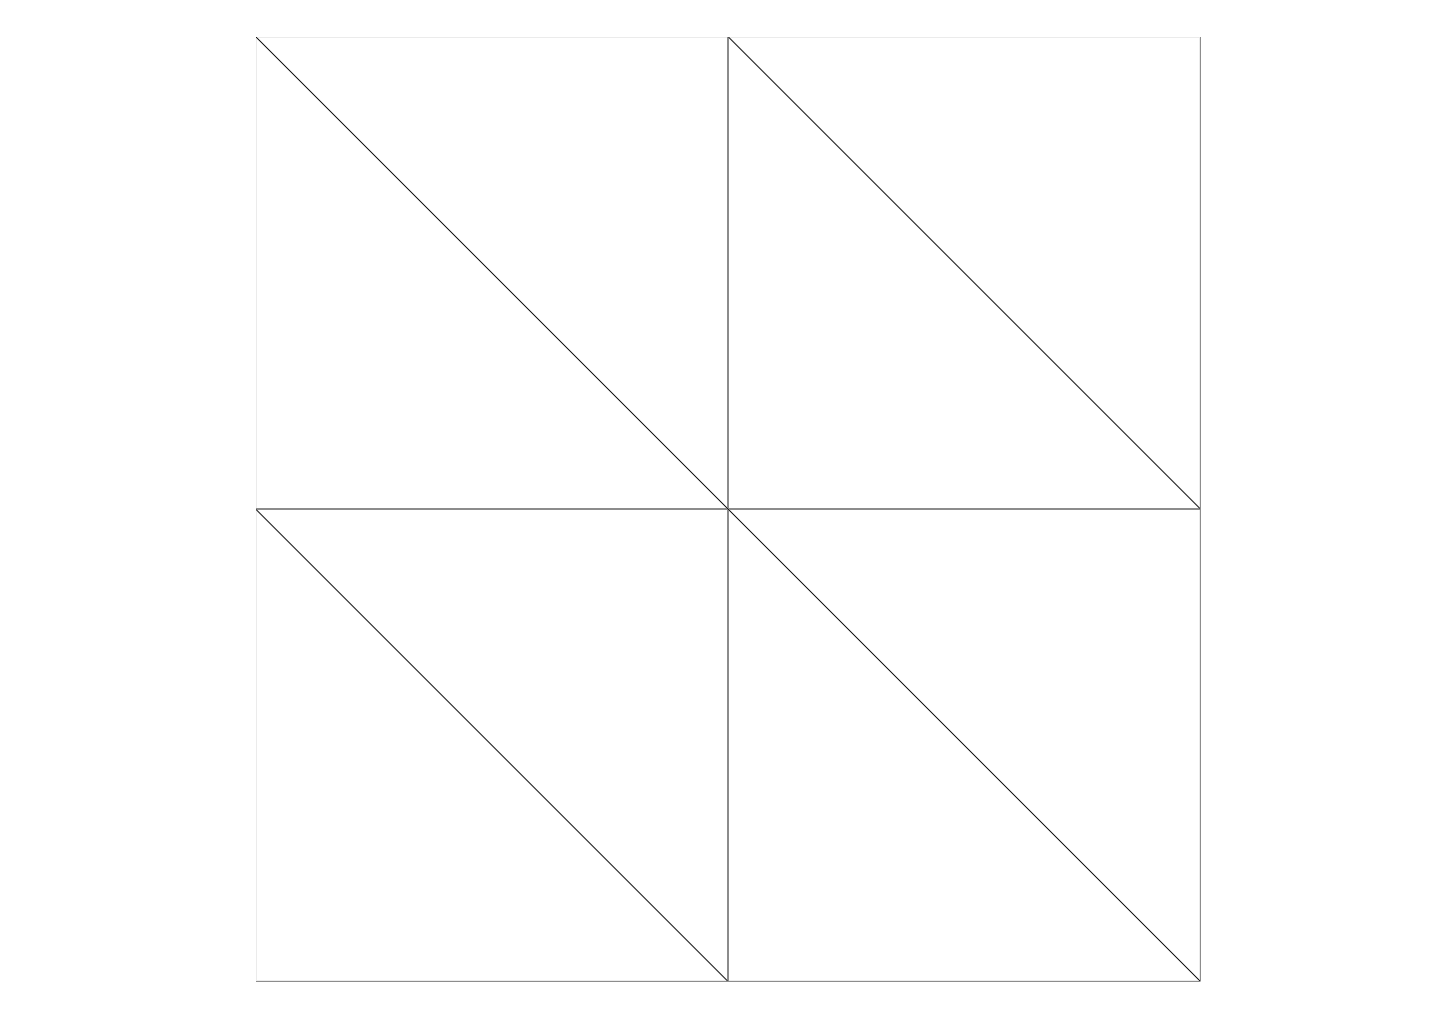
\includegraphics[width=.85\textwidth]{data/synthetic_meshes/square_tesselation_2tri_Dirac_delta_1_v9_f8_wireframe.png}
			{\footnotesize
				\par \vspace{-1mm} $r=1$,
				\par \vspace{-1mm} wireframe
			}
		\end{column}
		\begin{column}{0.22\textwidth}
			\centering
			
\includegraphics[width=.85\textwidth]{data/synthetic_meshes/square_tesselation_2tri_Dirac_delta_1_v9_f8_funcvals_0iter_crop.png}
			{\footnotesize
				\par \vspace{-1mm} $r=1$,
				\par \vspace{-1mm} $0$~iterations
			}
		\end{column}
		\begin{column}{0.22\textwidth}
			\centering
			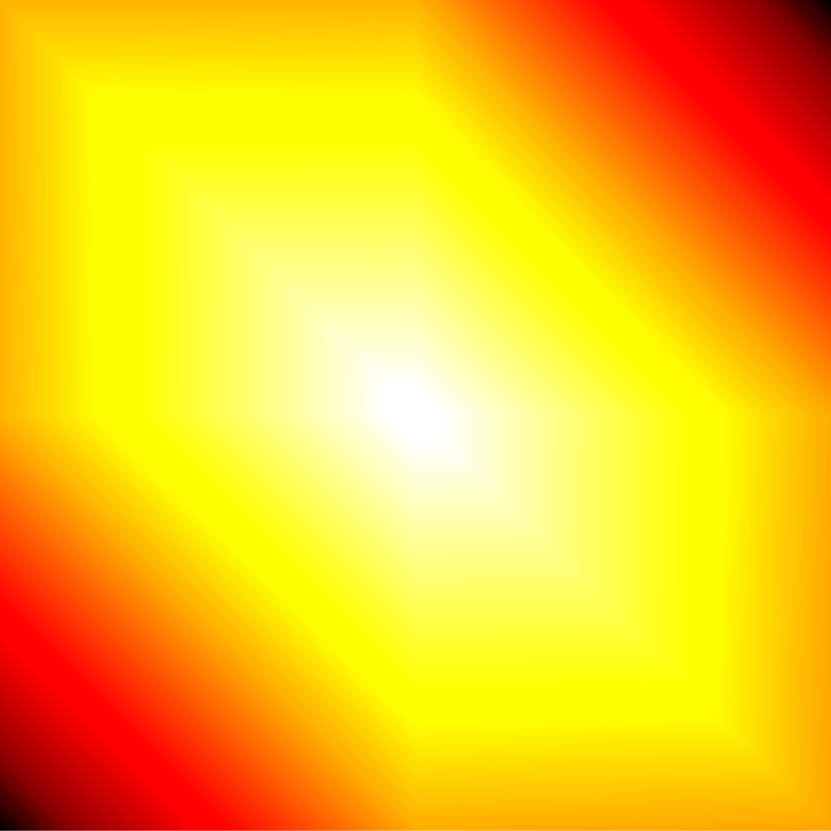
\includegraphics[width=.85\textwidth]{data/synthetic_meshes/square_tesselation_2tri_Dirac_delta_1_v9_f8_funcvals_1iter_crop.png}
			{\footnotesize
				\par \vspace{-1mm} $r=1$,
				\par \vspace{-1mm} $1$~iteration
			}
		\end{column}
		\begin{column}{0.17\textwidth}~\end{column}
	\end{columns}
	\vspace*{4mm}
	\begin{columns}
		\begin{column}{0.17\textwidth}~\end{column}
		\begin{column}{0.22\textwidth}
			\centering
			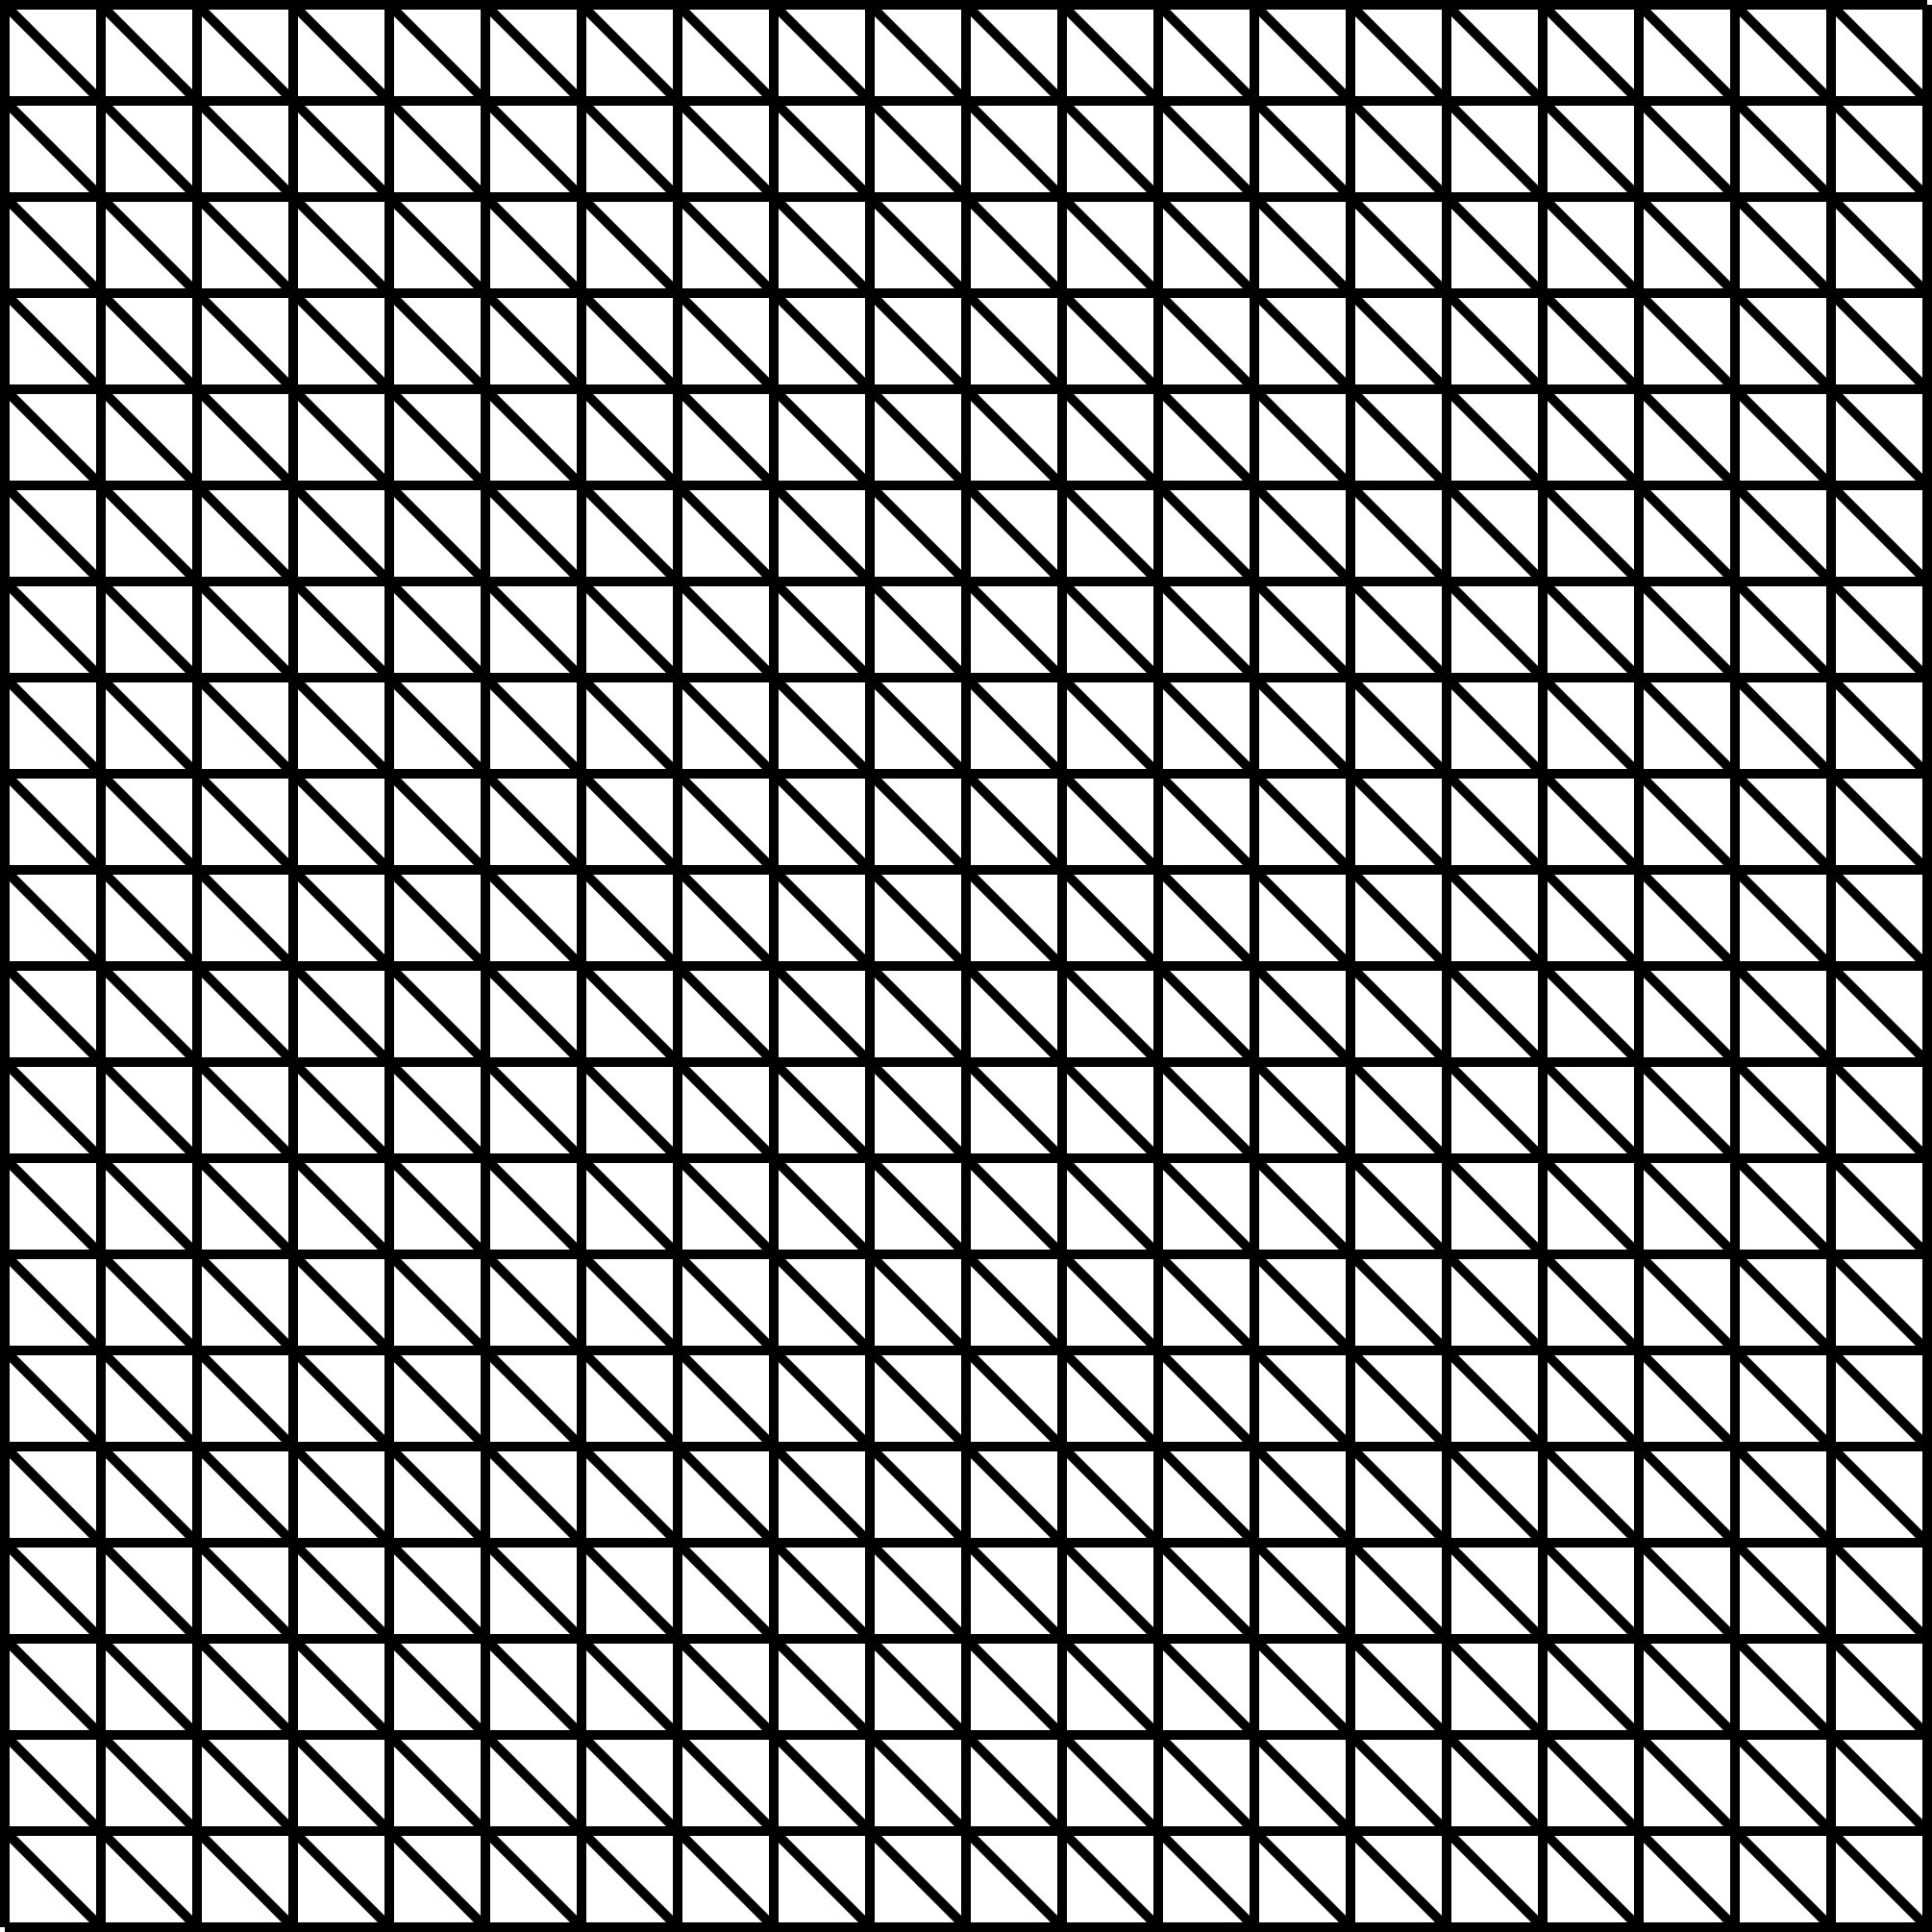
\includegraphics[width=.85\textwidth]{data/synthetic_meshes/square_tesselation_2tri_Dirac_delta_10_v441_f800_wireframe.png}
			{\footnotesize
				\par \vspace{-1mm} $r=10$,
				\par \vspace{-1mm} wireframe
			}
		\end{column}
		\begin{column}{0.22\textwidth}
			\centering
			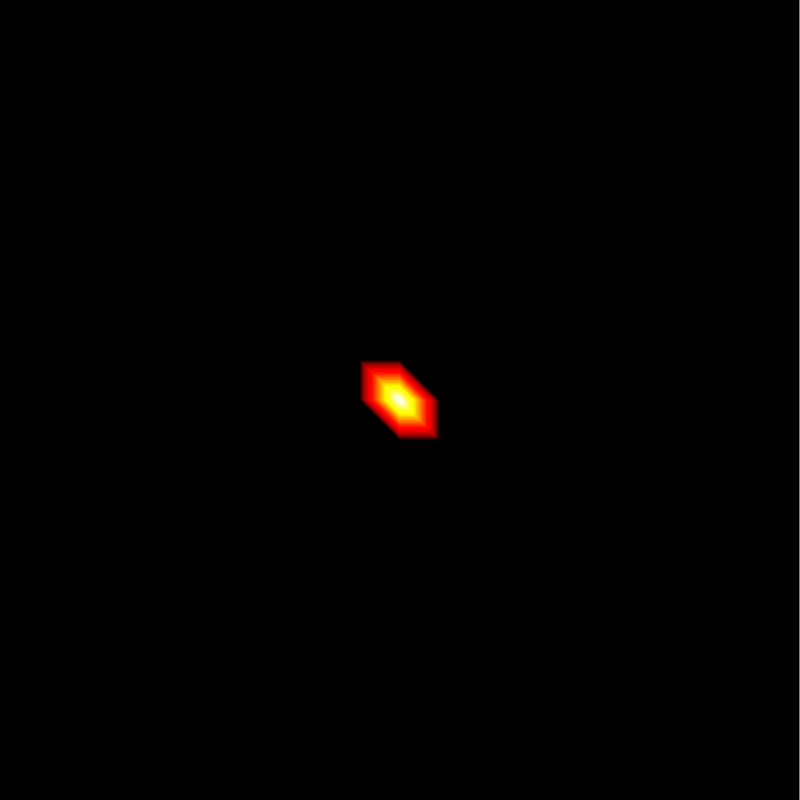
\includegraphics[width=.85\textwidth]{data/synthetic_meshes/square_tesselation_2tri_Dirac_delta_10_v441_f800_funcvals_0iter.png}
			{\footnotesize
				\par \vspace{-1mm} $r=10$,
				\par \vspace{-1mm} $0$~iterations
			}
		\end{column}
		\begin{column}{0.22\textwidth}
			\centering
			
\includegraphics[width=.85\textwidth]{data/synthetic_meshes/square_tesselation_2tri_Dirac_delta_10_v441_f800_funcvals_100iter.png}
			{\footnotesize
				\par \vspace{-1mm} $r=10$,
				\par \vspace{-1mm} $100$~iterations
			}
		\end{column}
		\begin{column}{0.17\textwidth}~\end{column}
	\end{columns}
}

%------------------------------------------------
\frame{\frametitle{Hexagonal Tessellations}
	\vspace*{-3mm}
	\begin{columns}
		\begin{column}{0.17\textwidth}~\end{column}
		\begin{column}{0.22\textwidth}
			\centering
			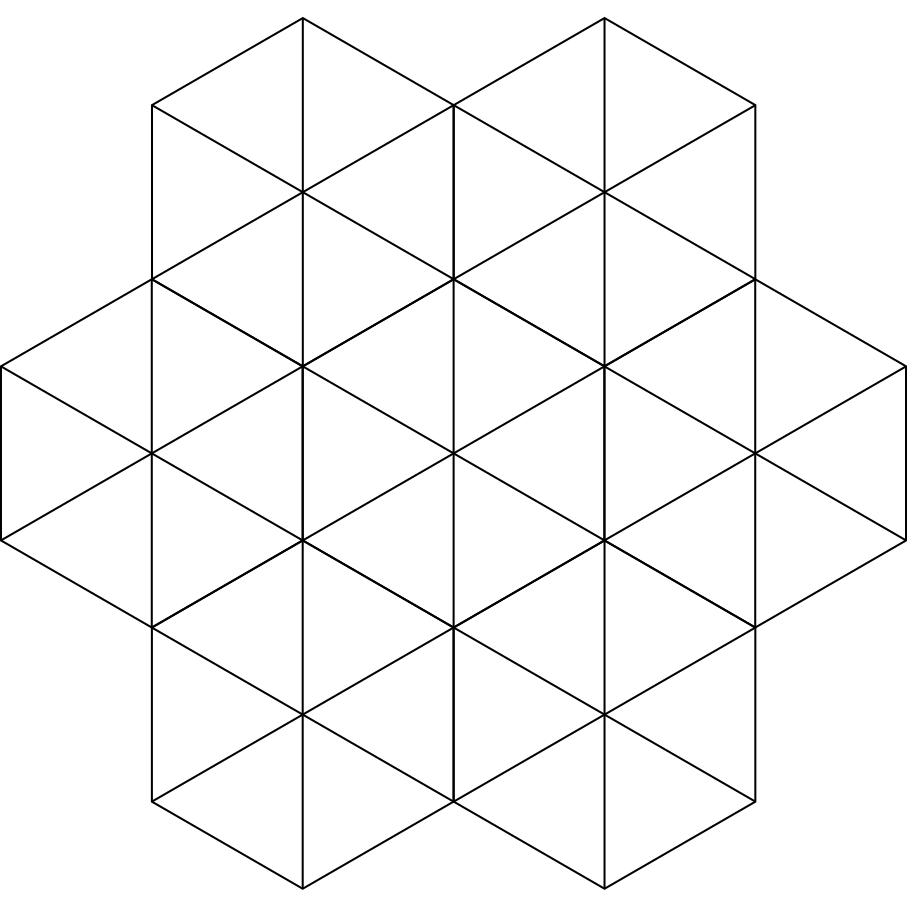
\includegraphics[width=.85\textwidth]{data/synthetic_meshes/hexagonal_tessellation_Dirac_delta_1_v31_f42_wireframe.png}
			{\footnotesize
				\par \vspace{-1mm} $r=1$,
				\par \vspace{-1mm} wireframe
			}
		\end{column}
		\begin{column}{0.22\textwidth}
			\centering
			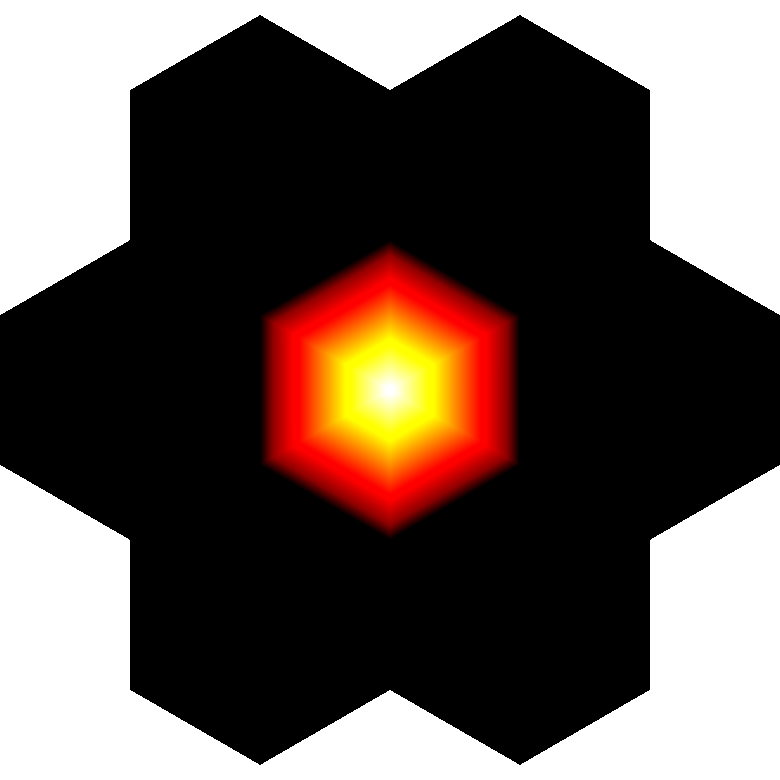
\includegraphics[width=.85\textwidth]{data/synthetic_meshes/hexagonal_tessellation_Dirac_delta_1_v31_f42_funcvals_0iter_crop.png}
			{\footnotesize
				\par \vspace{-1mm} $r=1$,
				\par \vspace{-1mm} $0$~iterations
			}
		\end{column}
		\begin{column}{0.22\textwidth}
			\centering
			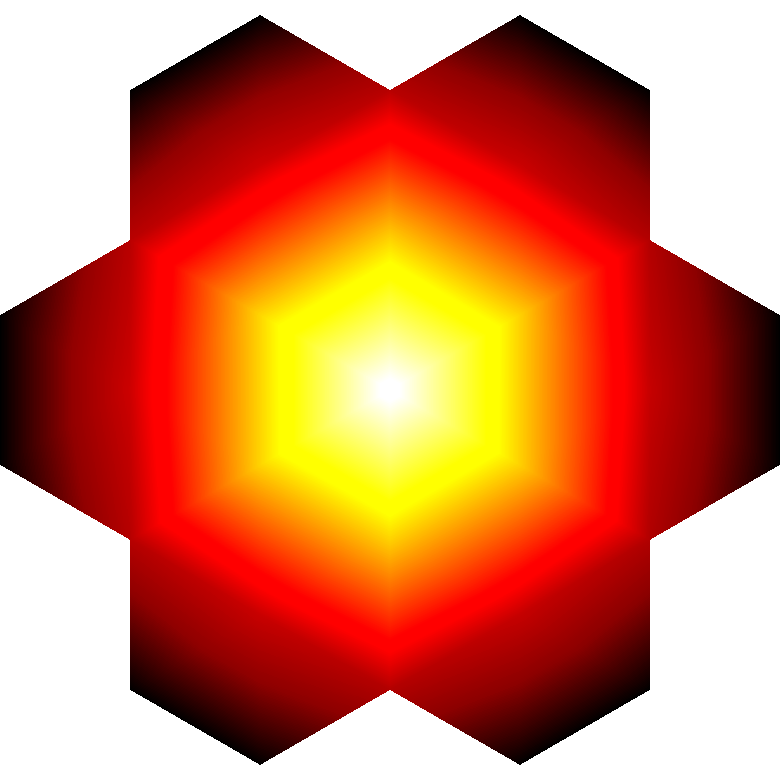
\includegraphics[width=.85\textwidth]{data/synthetic_meshes/hexagonal_tessellation_Dirac_delta_1_v31_f42_funcvals_2iter_crop.png}
			{\footnotesize
				\par \vspace{-1mm} $r=1$,
				\par \vspace{-1mm} $2$~iterations
			}
		\end{column}
		\begin{column}{0.17\textwidth}~\end{column}
	\end{columns}
	\vspace*{4mm}
	\begin{columns}
		\begin{column}{0.17\textwidth}~\end{column}
		\begin{column}{0.22\textwidth}
			\centering
			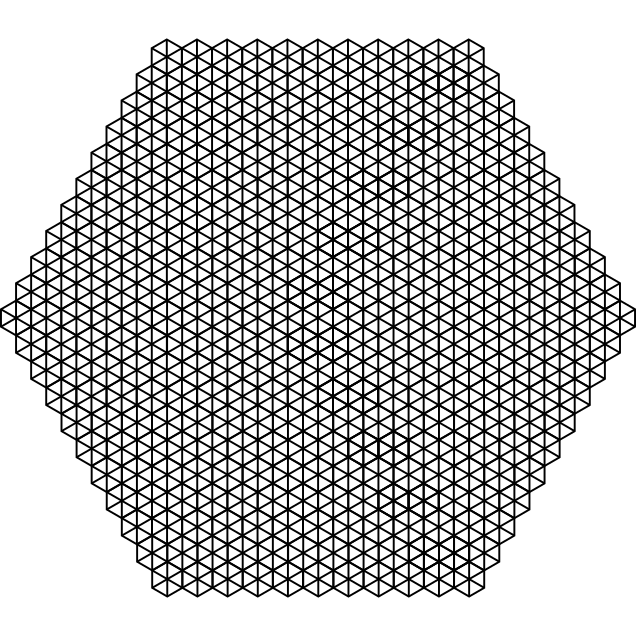
\includegraphics[width=.85\textwidth]{data/synthetic_meshes/hexagonal_tessellation_Dirac_delta_10_v1057_f1986_wireframe.png}
			{\footnotesize
				\par \vspace{-1mm} $r=10$,
				\par \vspace{-1mm} wireframe
			}
		\end{column}
		\begin{column}{0.22\textwidth}
			\centering
			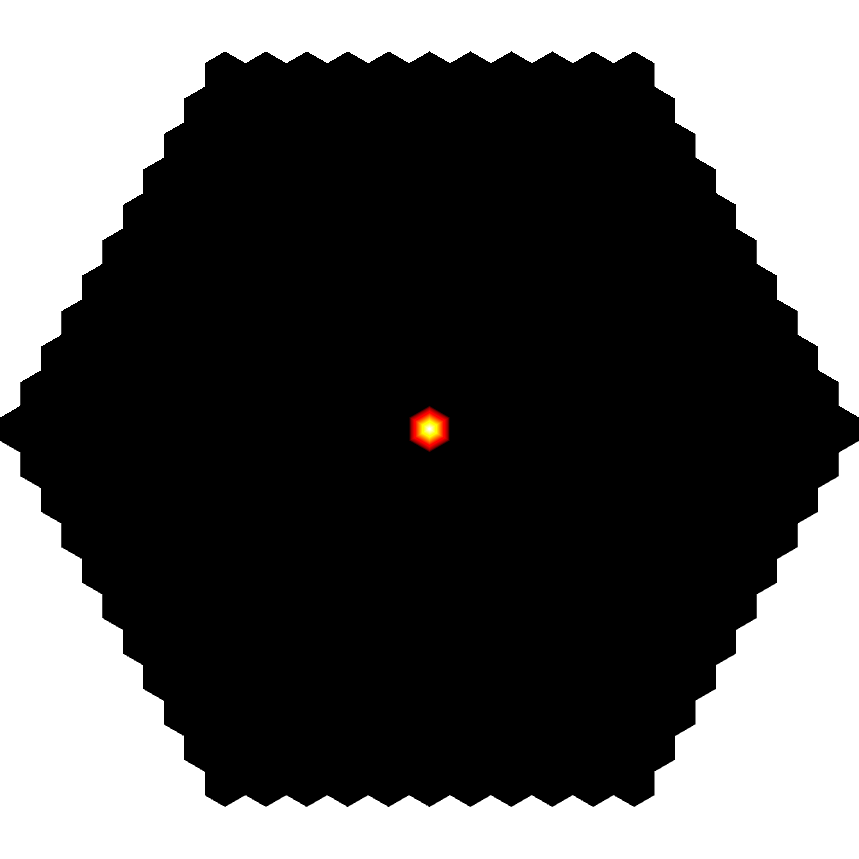
\includegraphics[width=.85\textwidth]{data/synthetic_meshes/hexagonal_tessellation_Dirac_delta_10_v1057_f1986_funcvals_0iter_crop.png}
			{\footnotesize
				\par \vspace{-1mm} $r=10$,
				\par \vspace{-1mm} $0$~iterations
			}
		\end{column}
		\begin{column}{0.22\textwidth}
			\centering
			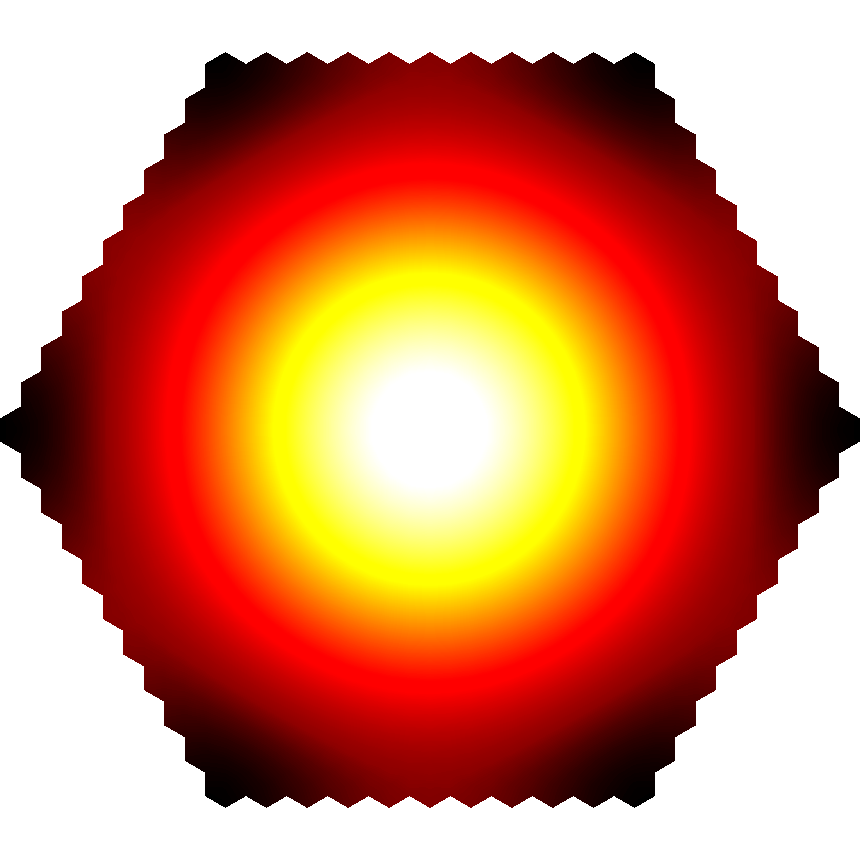
\includegraphics[width=.85\textwidth]{data/synthetic_meshes/hexagonal_tessellation_Dirac_delta_10_v1057_f1986_funcvals_200iter_crop.png}
			{\footnotesize
				\par \vspace{-1mm} $r=10$,
				\par \vspace{-1mm} $200$~iterations
			}
		\end{column}
		\begin{column}{0.17\textwidth}~\end{column}
	\end{columns}
}

%------------------------------------------------
\frame{\frametitle{Random Triangulated Discs}
	\vspace*{-3mm}
	\begin{columns}
		\begin{column}{0.17\textwidth}~\end{column}
		\begin{column}{0.22\textwidth}
			\centering
			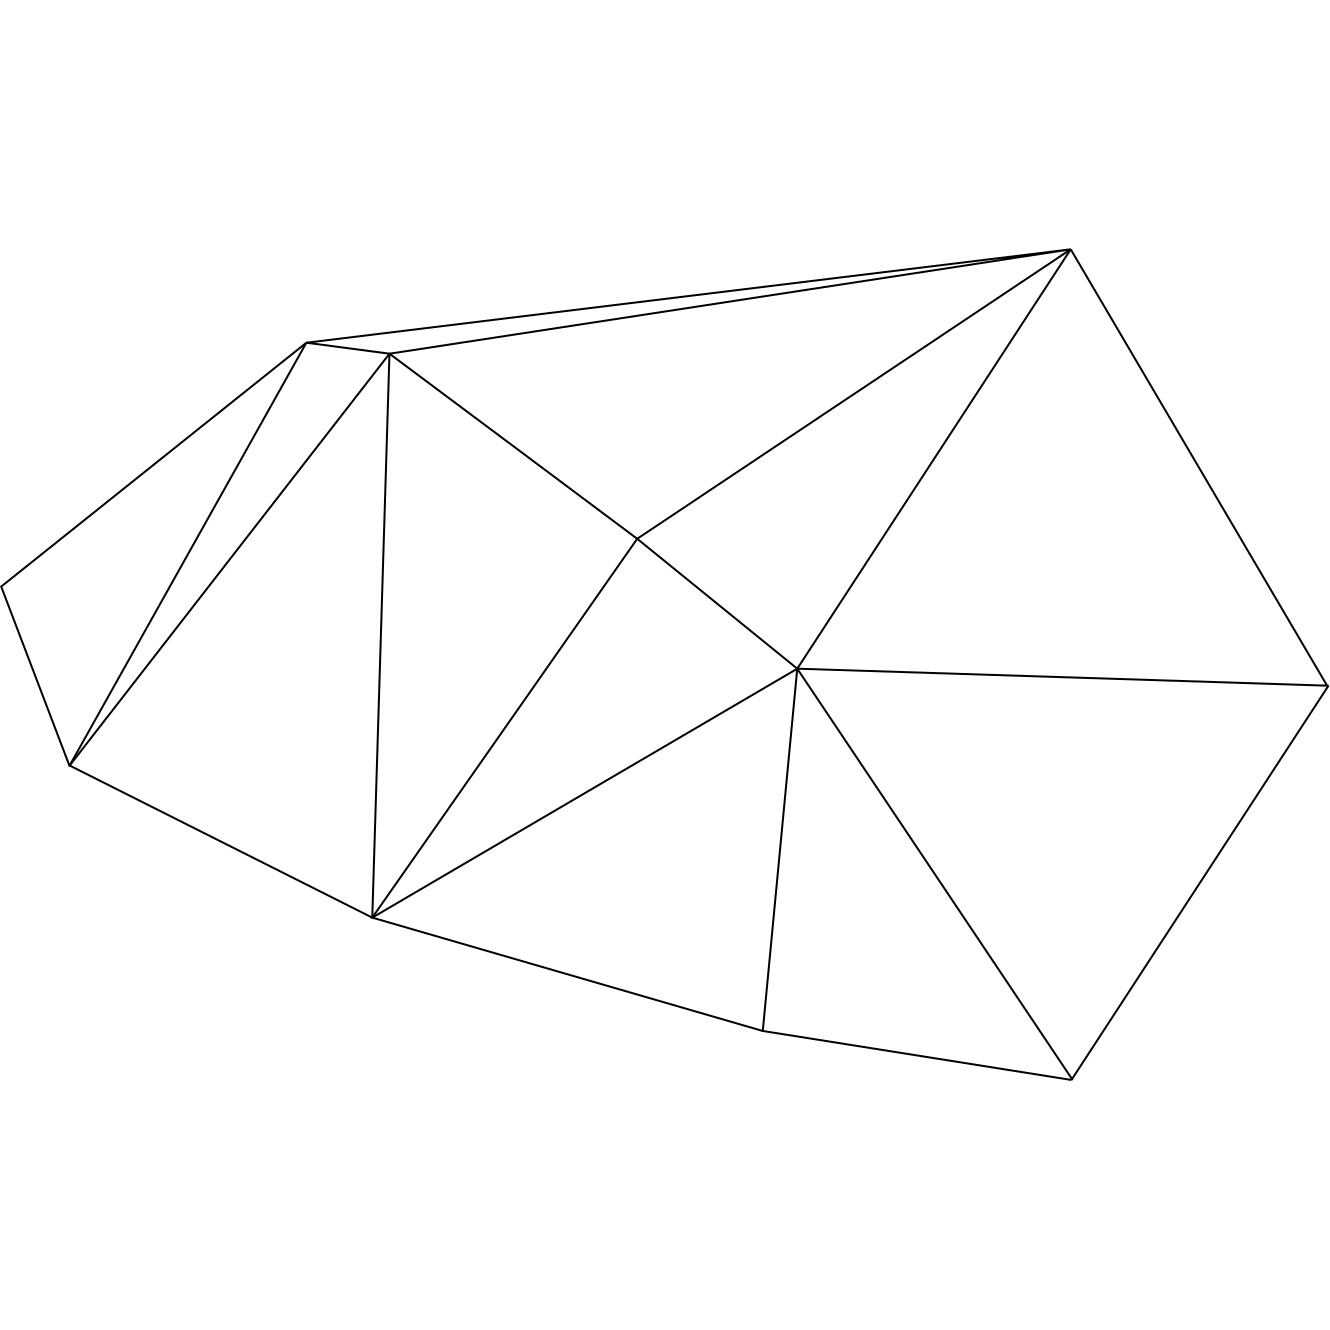
\includegraphics[width=.85\textwidth]{data/synthetic_meshes/random_circle_tessellation_Dirac_delta_1_v11_f12_wireframe.png}
			{\footnotesize
				\par \vspace{-1mm} $r=1$, $p=11$,
				\par \vspace{-1mm} wireframe
			}
		\end{column}
		\begin{column}{0.22\textwidth}
			\centering
			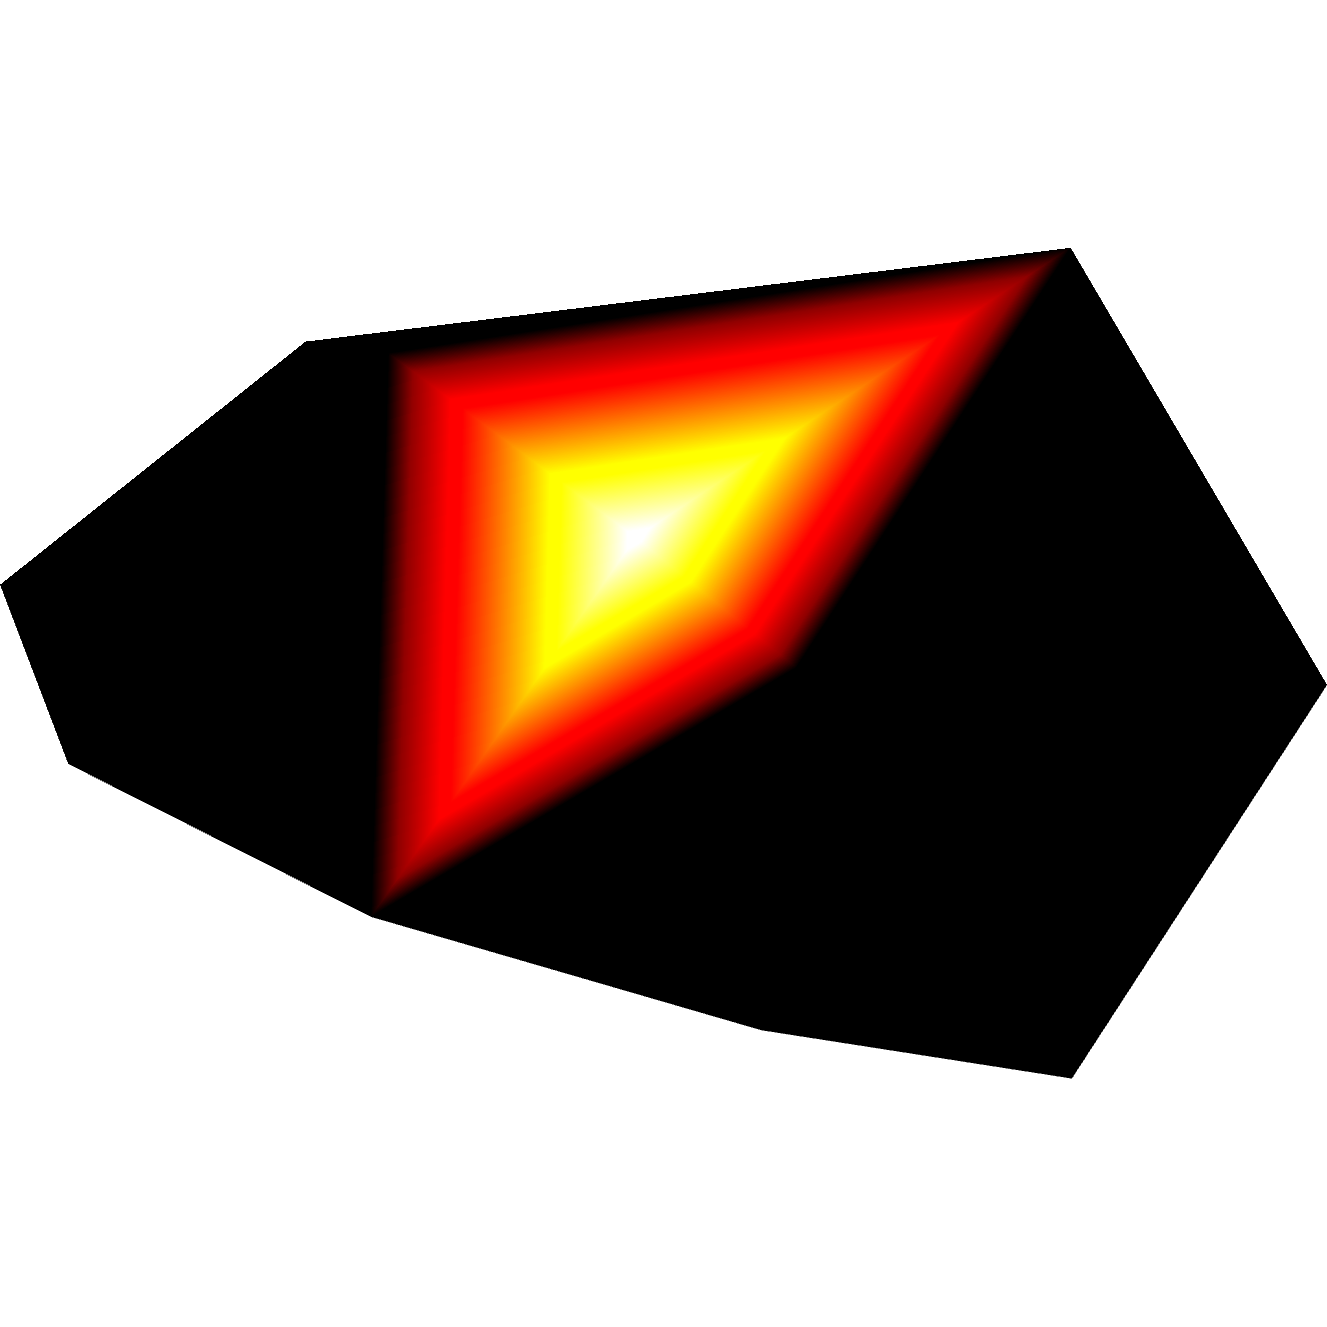
\includegraphics[width=.85\textwidth]{data/synthetic_meshes/random_circle_tessellation_Dirac_delta_1_v11_f12_funcvals_0iter.png}
			{\footnotesize
				\par \vspace{-1mm} $r=1$, $p=11$,
				\par \vspace{-1mm} $0$~iterations
			}
		\end{column}
		\begin{column}{0.22\textwidth}
			\centering
			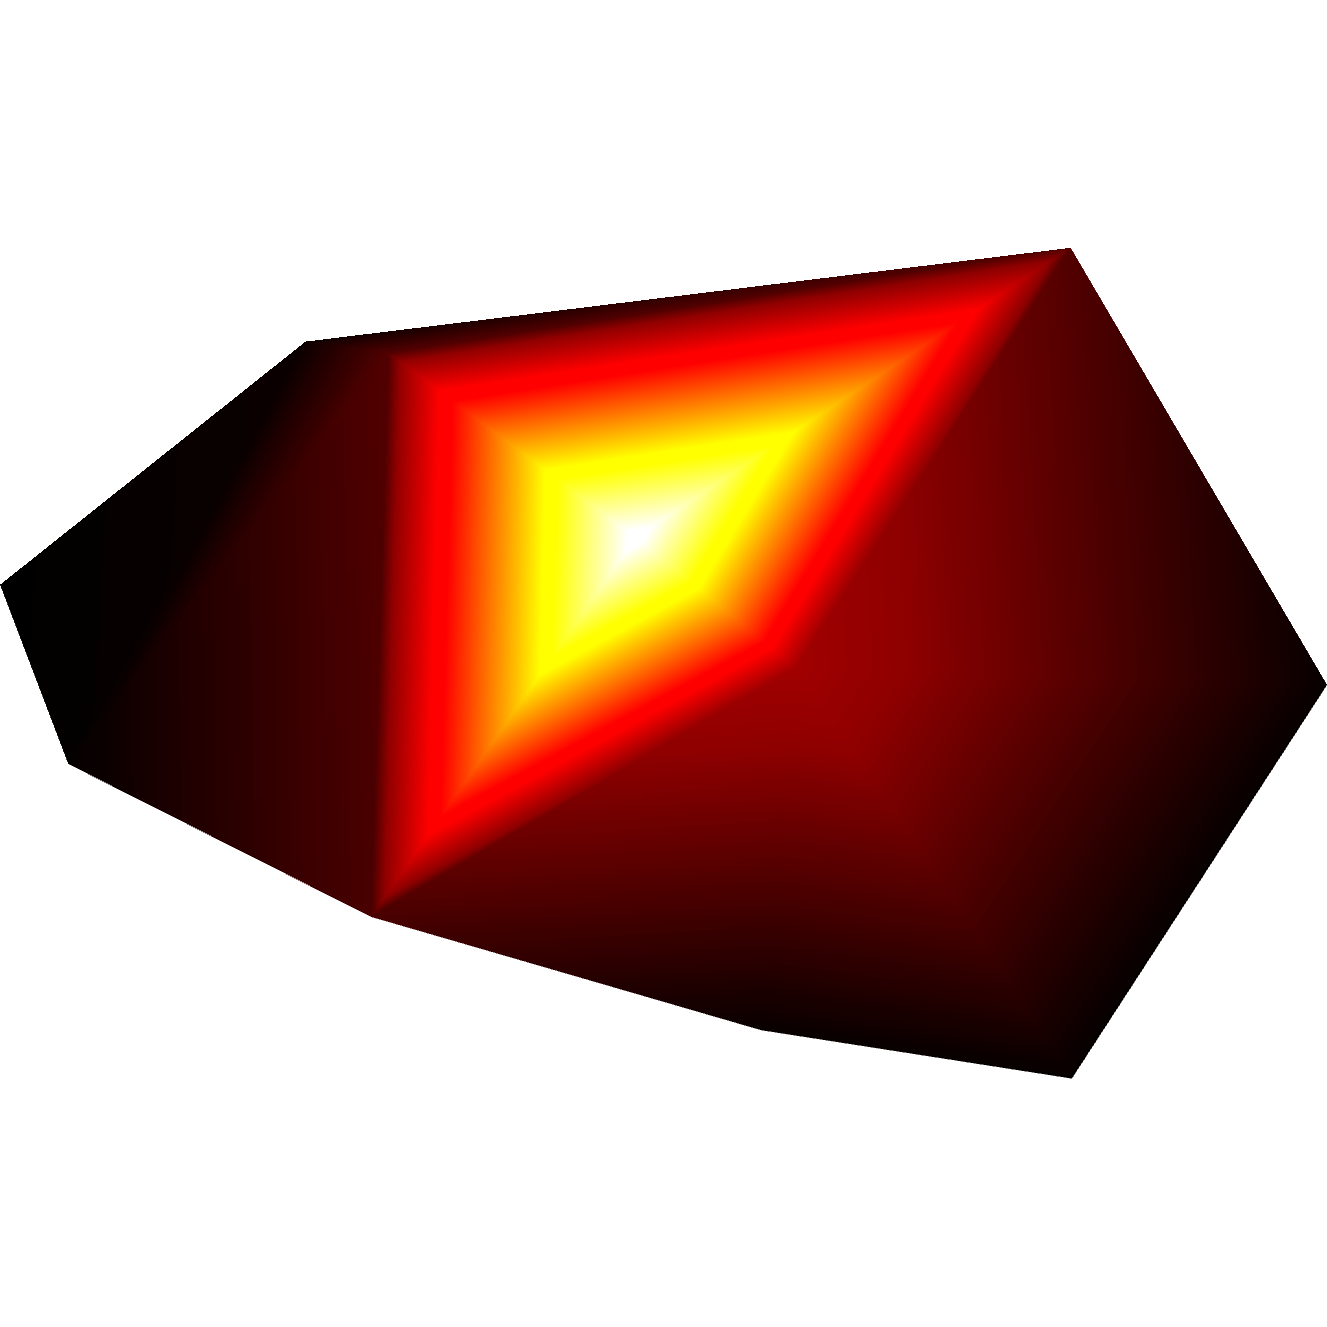
\includegraphics[width=.85\textwidth]{data/synthetic_meshes/random_circle_tessellation_Dirac_delta_1_v11_f12_funcvals_2iter.png}
			{\footnotesize
				\par \vspace{-1mm} $r=1$, $p=11$,
				\par \vspace{-1mm} $2$~iterations
			}
		\end{column}
		\begin{column}{0.17\textwidth}~\end{column}
	\end{columns}
	\vspace*{4mm}
	\begin{columns}
		\begin{column}{0.17\textwidth}~\end{column}
		\begin{column}{0.22\textwidth}
			\centering
			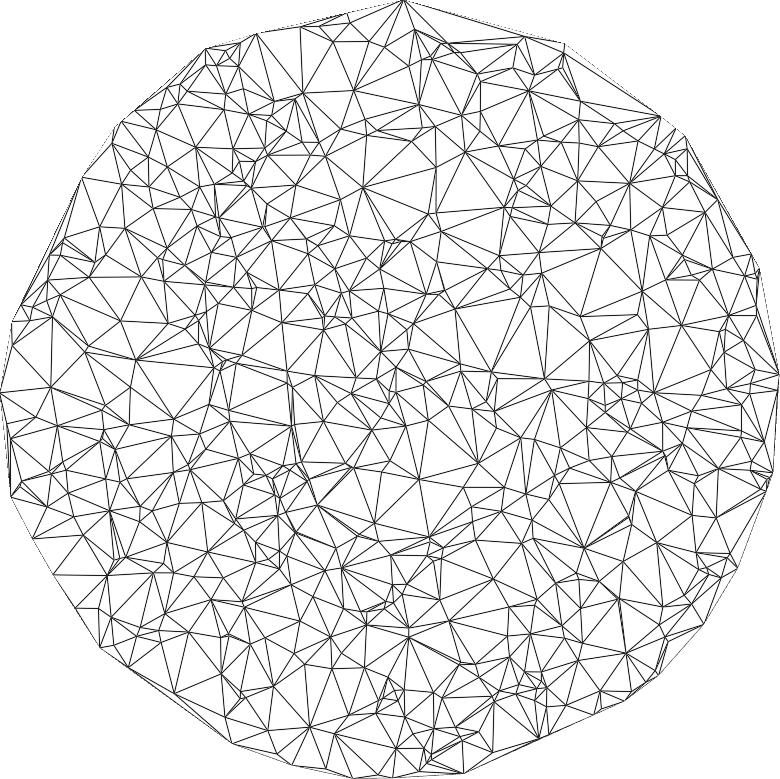
\includegraphics[width=.85\textwidth]{data/synthetic_meshes/random_circle_tessellation_Dirac_delta_10_v641_f1252_wireframe.png}
			{\footnotesize
				\par \vspace{-1mm} $r=10$, $p=641$,
				\par \vspace{-1mm} wireframe
			}
		\end{column}
		\begin{column}{0.22\textwidth}
			\centering
			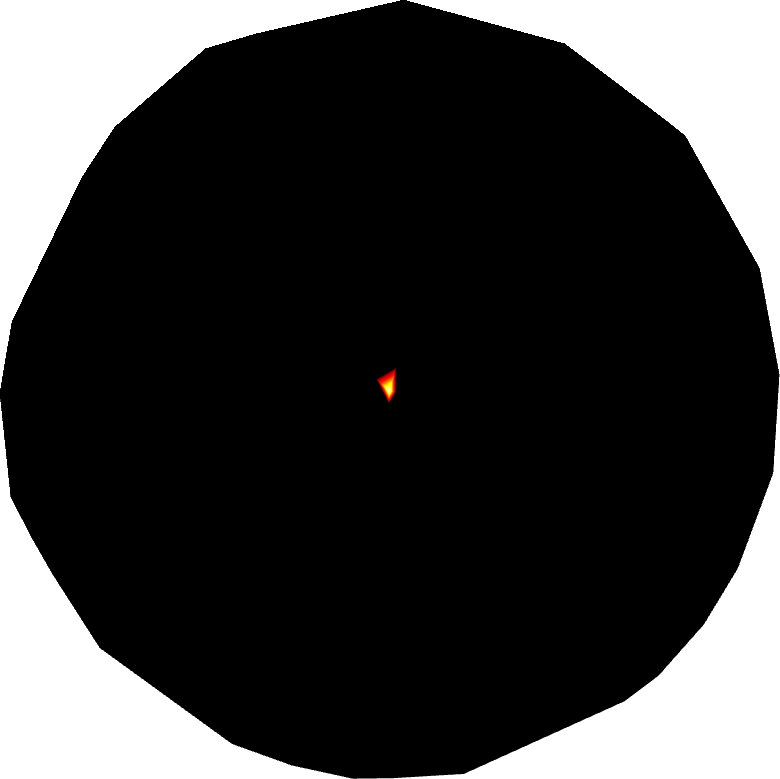
\includegraphics[width=.85\textwidth]{data/synthetic_meshes/random_circle_tessellation_Dirac_delta_10_v641_f1252_funcvals_0iter.png}
			{\footnotesize
				\par \vspace{-1mm} $r=10$, $p=641$,
				\par \vspace{-1mm} $0$~iterations
			}
		\end{column}
		\begin{column}{0.22\textwidth}
			\centering
			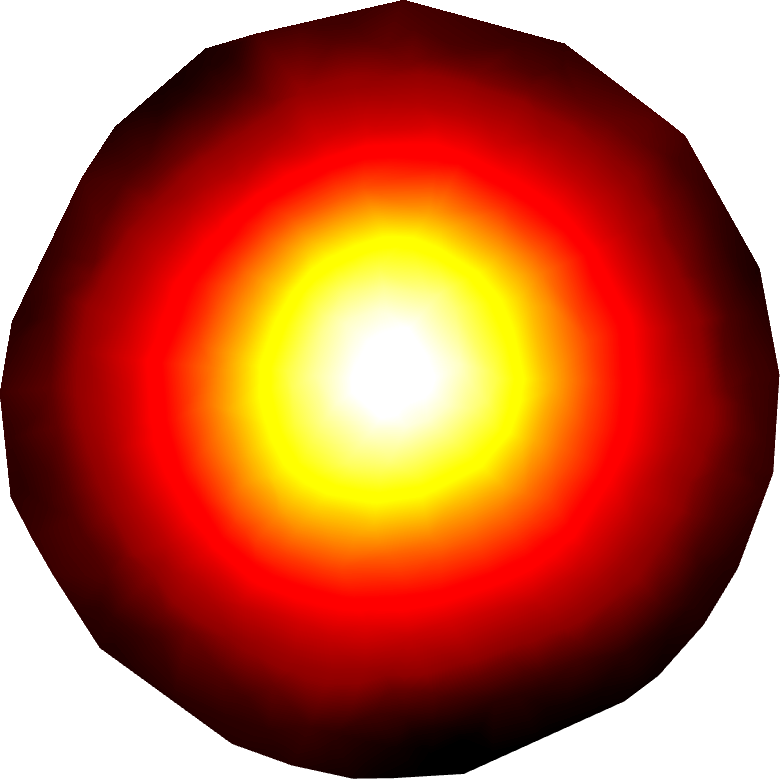
\includegraphics[width=.85\textwidth]{data/synthetic_meshes/random_circle_tessellation_Dirac_delta_10_v641_f1252_funcvals_10000iter.png}
			{\footnotesize
				\par \vspace{-1mm} $r=10$, $p=641$,
				\par \vspace{-1mm} $10^4$~iterations
			}
		\end{column}
		\begin{column}{0.17\textwidth}~\end{column}
	\end{columns}
}

%------------------------------------------------
%TODO:callout errors
\frame{\frametitle{The University of Heidelberg Seal}
	%\vspace*{2mm}
	%\begin{flushright}error propagation\par\end{flushright}
	%\vspace*{4mm}
	\vspace*{16mm}
	\begin{columns}
		\begin{column}{0.33\textwidth}
			\centering
			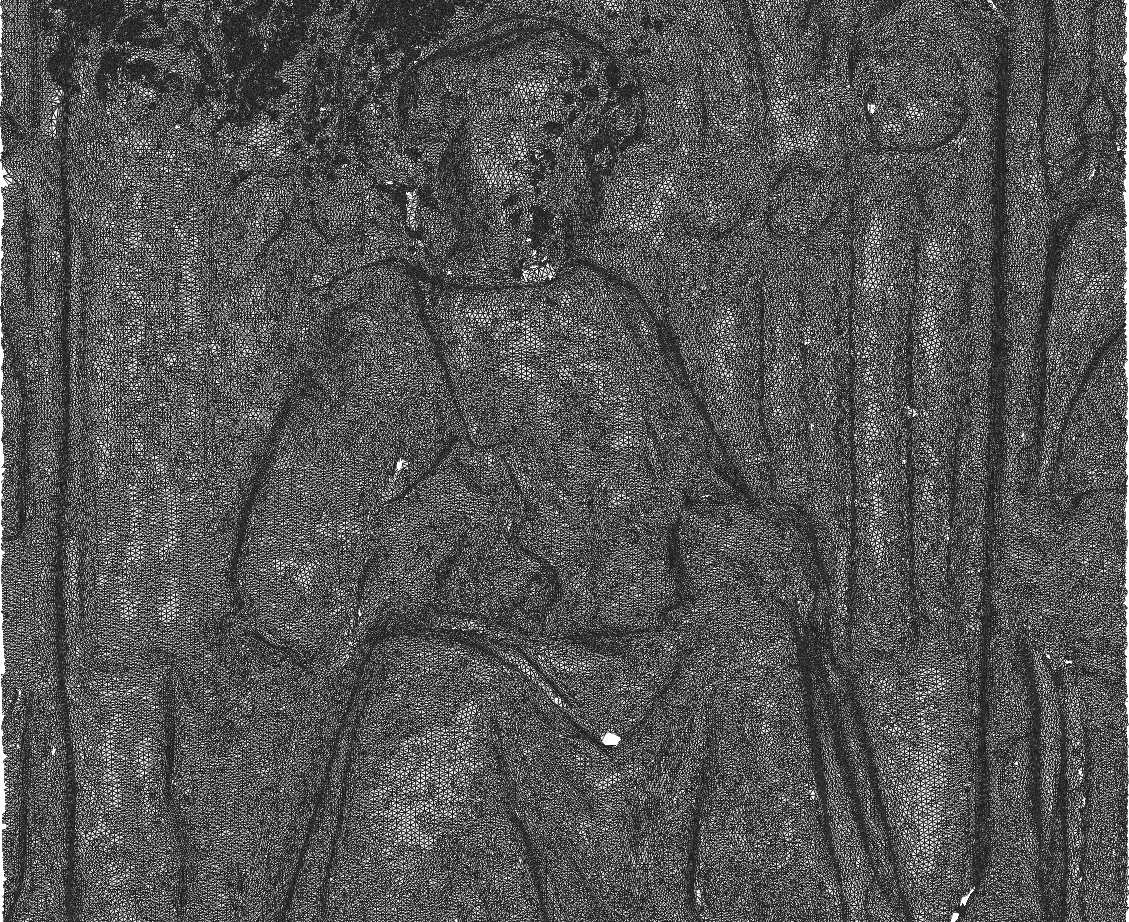
\includegraphics[width=\textwidth]{data/acquired_meshes/unisiegel_wireframe.png}
			{\footnotesize
				\par \vspace{-1mm} wireframe
			}
		\end{column}
		\begin{column}{0.33\textwidth}
			\centering
			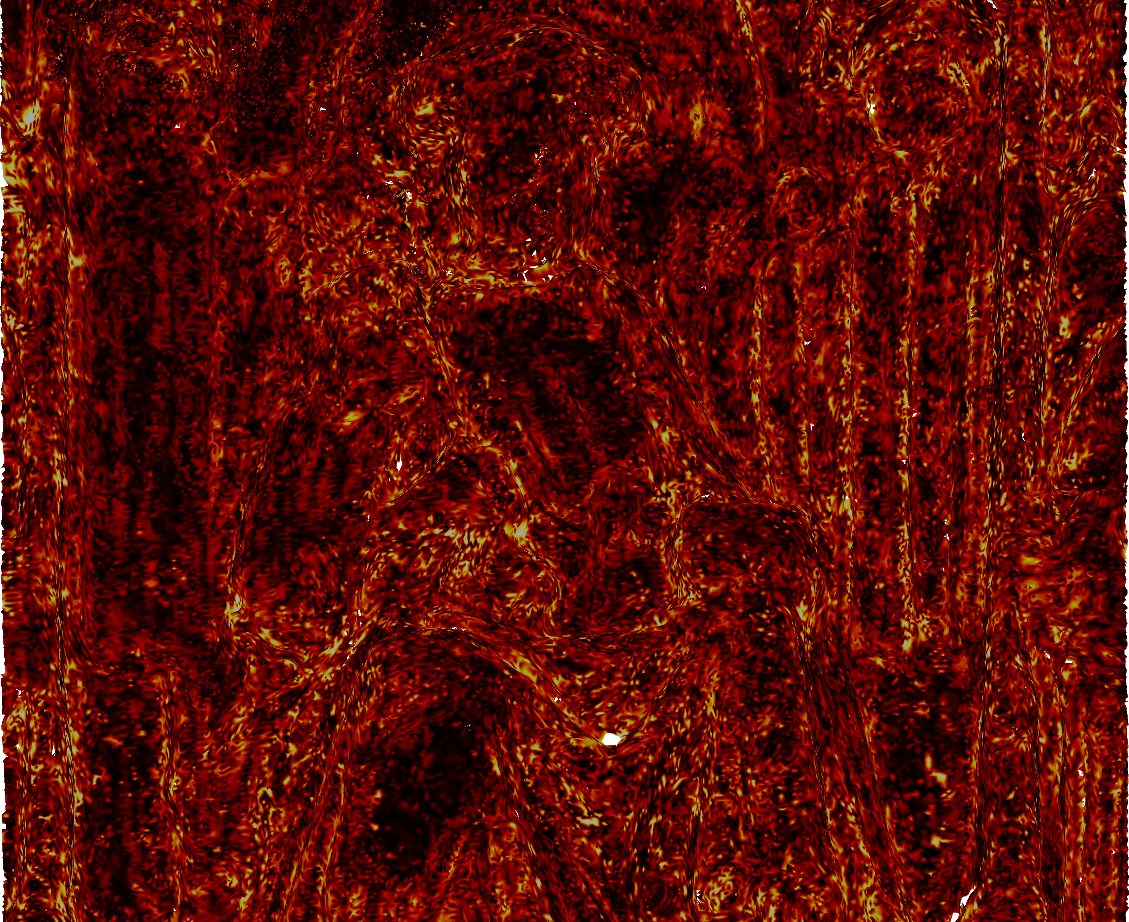
\includegraphics[width=\textwidth]{data/acquired_meshes/unisiegel_0iter.png}
			{\footnotesize
				\par \vspace{-1mm} $0$~iterations
			}
		\end{column}
		\begin{column}{0.33\textwidth}
			\centering
			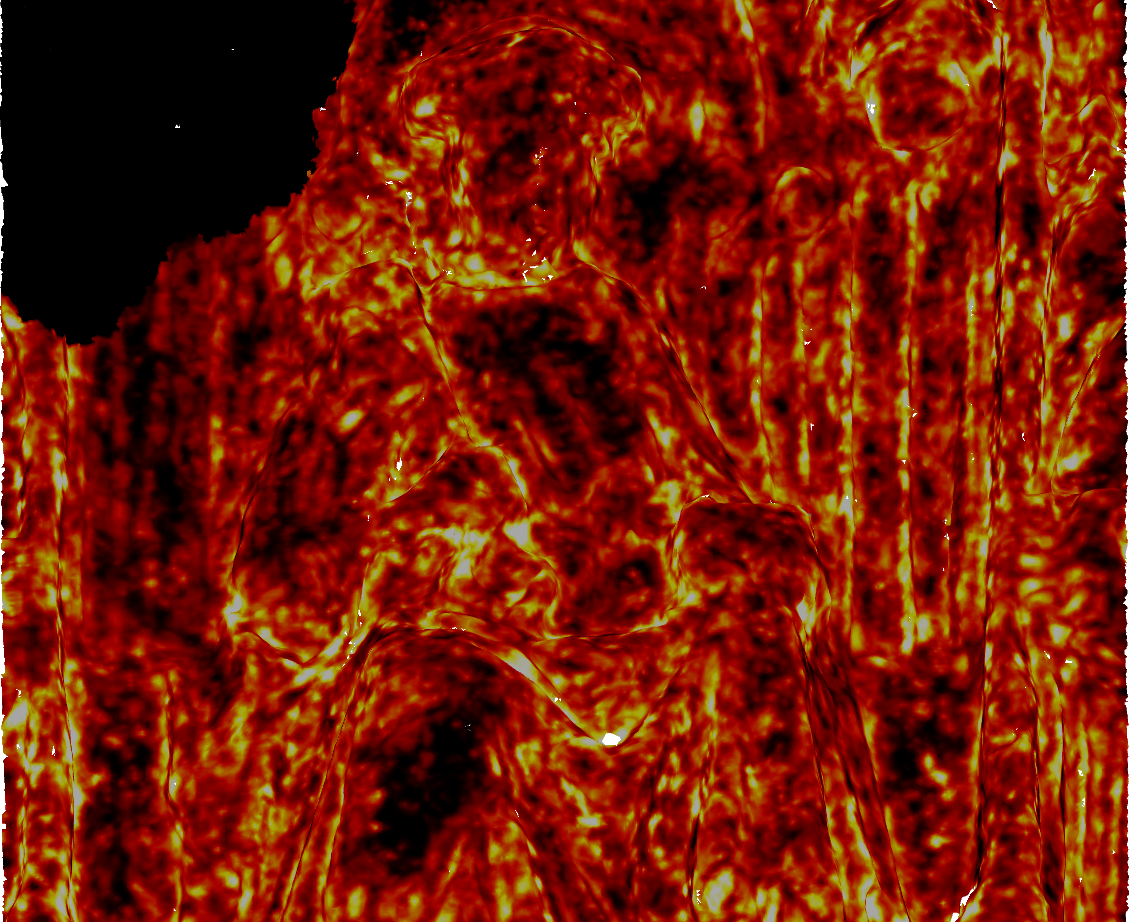
\includegraphics[width=\textwidth]{data/acquired_meshes/unisiegel_100iter.png}
			{\footnotesize
				\par \vspace{-1mm} $100$~iterations
			}
		\end{column}
	\end{columns}
	%\begin{tikzpicture}[overlay, remember picture]
	%	\draw[gray,ultra thick] (36mm, 70mm) -- (60mm, 71mm);
	%\end{tikzpicture}
}

%------------------------------------------------
\frame{\frametitle{A flat surface from ILATO}
	\vspace*{-2mm}
	\begin{columns}
		\begin{column}{0.5\textwidth}
			\centering
			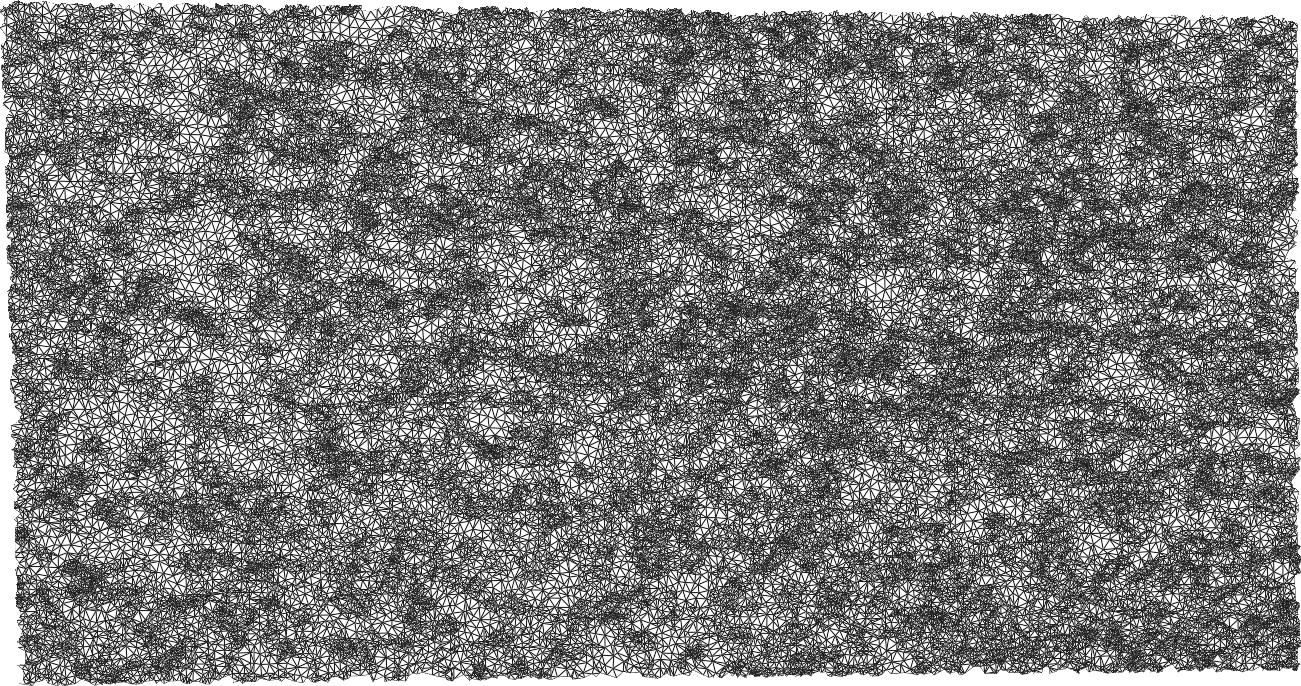
\includegraphics[width=.75\textwidth]{data/acquired_meshes/ILATO_1A_SM2066-HE5-60_070214_merged_GMO_r1_n4_v256_wireframe.png}
			{\footnotesize
				\par \vspace{-1mm} wireframe
			}
		\end{column}
		\begin{column}{0.5\textwidth}
			\centering
			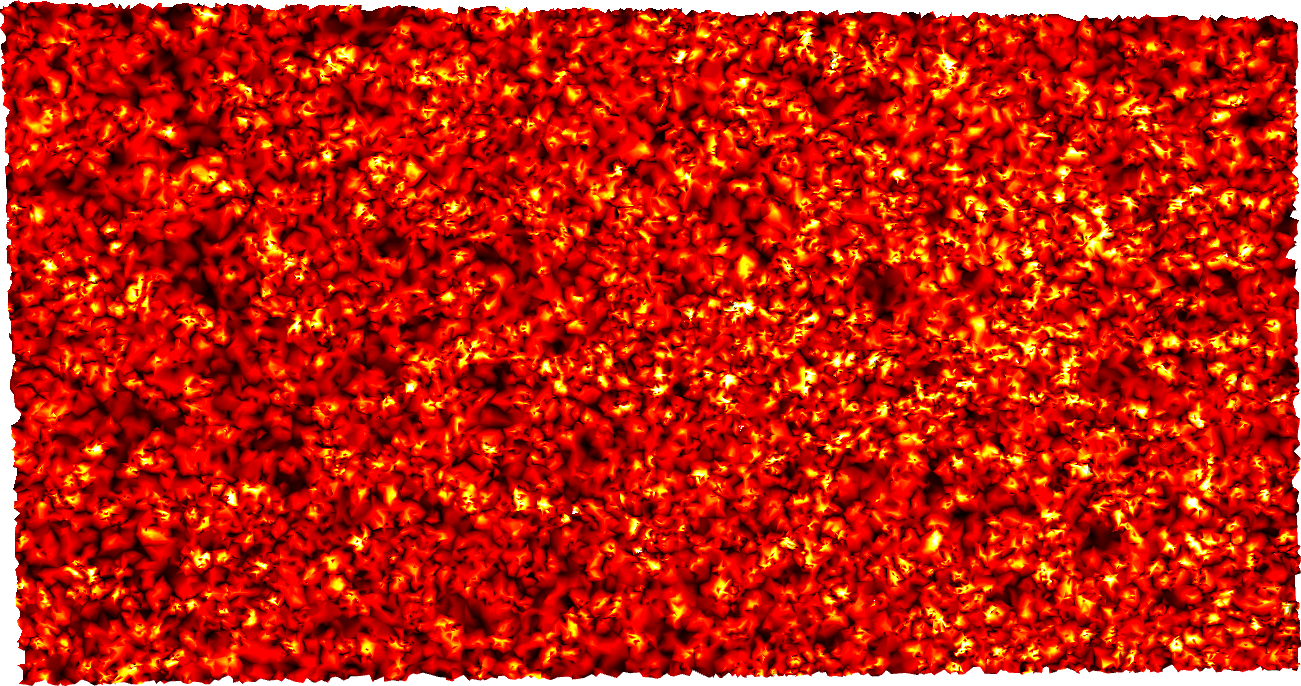
\includegraphics[width=.75\textwidth]{data/acquired_meshes/ILATO_1A_SM2066-HE5-60_070214_merged_GMO_r1_n4_v256_funcvals_0iter.png}
			{\footnotesize
				\par \vspace{-1mm} $0$~iterations
			}
		\end{column}
	\end{columns}
	\vspace*{4mm}
	\begin{columns}
		\begin{column}{0.5\textwidth}
			\centering
			\includegraphics[width=.75\textwidth]{data/acquired_meshes/ILATO_1A_SM2066-HE5-60_070214_merged_GMO_r1_n4_v256_funcvals_1000iter.png}
			{\footnotesize
				\par \vspace{-1mm} $1000$~iterations
			}
		\end{column}
		\begin{column}{0.5\textwidth}
			\centering
			\includegraphics[width=.75\textwidth]{data/acquired_meshes/ILATO_1A_SM2066-HE5-60_070214_merged_GMO_r1_n4_v256_funcvals_3000iter.png}
			{\footnotesize
				\par \vspace{-1mm} $3000$~iterations
			}
		\end{column}
	\end{columns}
}

%------------------------------------------------
\frame{\frametitle{The Stanford Bunny}
	\vspace*{8mm}
	\begin{columns}
		\begin{column}{0.33\textwidth}
			\centering
			\includegraphics[width=\textwidth]{data/acquired_meshes/bun_zipper_edited_r1_n4_v256_wireframe.png}
			{\footnotesize
				\par \vspace{-1mm} wireframe
			}
		\end{column}
		\begin{column}{0.33\textwidth}
			\centering
			\includegraphics[width=\textwidth]{data/acquired_meshes/bun_zipper_edited_r1_n4_v256_funcvals_0iter.png}
			{\footnotesize
				\par \vspace{-1mm} $0$~iterations
			}
		\end{column}
		\begin{column}{0.33\textwidth}
			\centering
			\includegraphics[width=\textwidth]{data/acquired_meshes/bun_zipper_edited_r1_n4_v256_funcvals_100iter.png}
			{\footnotesize
				\par \vspace{-1mm} $100$~iterations
			}
		\end{column}
	\end{columns}
}


%================================================
\subsection{Performance utilizing \glspl{GPGPU}}

%------------------------------------------------
\frame{\frametitle{Compute Times per Experiment for increasing Iteration Counts}
	\vspace*{-2mm}
	{\centering
	\includegraphics[width=1.0\textwidth]{figures/computeTimesLinespoints_presentation.png}}
	\only<2>{
		\par \vspace*{-20mm}
		\begin{flushright}\emph{\LARGE Predictable!}\end{flushright}
	}
	\begin{tikzpicture}[overlay, remember picture]
		\draw<2>[black,ultra thick,rounded corners] (52mm, 68mm) rectangle (109mm, 3.5mm);
	\end{tikzpicture}
}

%------------------------------------------------
\frame{\frametitle{Compute Times Scatter Plot}
	\vspace*{-3mm}
	\centering
	\includegraphics[width=.72\textwidth]{figures/computeTimesScatter_presentation.png}
}

%------------------------------------------------

\frame{\frametitle{Speedup:~~~$\mathit{S}(\hat{n},\,\rho) = \mathit{T_s}(\hat{n}) \mathbin{/} \mathit{T_{\rho}}(\hat{n},\,\rho)$}
	\vspace*{-3mm}
	\centering
	\includegraphics[width=.9\textwidth]{figures/speedup.png}
}

%------------------------------------------------
\frame{\frametitle{Efficiency~~~$\mathit{E}(\hat{n},\,\rho) = \mathit{S}(\hat{n},\,\rho) \mathbin{/} \rho$}
	\vspace*{-3mm}
	\centering
	\includegraphics[width=.9\textwidth]{figures/efficiency.png}
}




%================================================
%================================================
\section[Outlook]{Outlook}

%------------------------------------------------
\frame{\frametitle{Outlook}
	\begin{columns}
		\begin{column}{.6\textwidth}
			\only<1->{
				\color{unirot}{Fast One-Ring Smoothing Filter:}
				\begin{itemize}
					\item Using inner angles vs area for weights
					\item Define a parameter instead of ${\color{MyTeal}\gelm}$%min edge length, discoverd by typo in original code
					%\item Eliminate square root function %no averaging, interpolation
					\item Other smoothing methods, i.e. median
				\end{itemize}
			}\only<2->{
				\vspace*{4mm}
				\color{unirot}{Parallelization:}
				\begin{itemize}
					\item Explicitly support feature vectors
					\item Use OpenCL to support other GPGPUs
				\end{itemize}
			}
		\end{column}
		\begin{column}{.2\textwidth}
			\only<3>{
				\par \vspace*{12mm}
				{\fontfamily{pzc}\selectfont
					\Huge
					Thank \par
					\begin{flushright}You!\end{flushright}
				}
			}
		\end{column}
	\end{columns}
}
%\fi
\end{document}
